\cotefile{137}
\scanpage{2}
% archive foliation: 1
\margin{\unsure{le même} \illegible{3}; \unsure{$k_*$} \illegible{5}}

\uline{Lemme 1} Soit $L_*$ un $k$-module $\frac12$ \unsure{simplicial}.
Pour que $L_*$ soit un \unsure{$k_*$-module} projectif, il suffit
qu'il soit flasque (i.e. $\unsure{\pi_i}(L_*)=0$ $\forall i\geq 0$), et que
les $L_n$ soient des $k$-modules projectifs.
\margin{\unsure{NB} \illegible{2} \unsure{$L_*$} \illegible{3} \unsure{projectif}}

La \unsure{cond°} \illegible{1} \unsure{signifie aussi} que le complexe de
chaînes (de $k$-modules) associé par Dold-Puppe
est acyclique et à \unsure{composantes projectives}. On voit
alors qu'il est \inserted{\unsure{donc}} isomorphe à une somme directe
\unsure{de complexes de chaînes de la forme}
\[
\unsure{0\longrightarrow L\xrightarrow{\mathrm{id}}L\longrightarrow 0}.
\]
\unsure{On} \illegible{3} \unsure{tel}
\illegible{2} \unsure{correspond} \illegible{4}
\unsure{complexe} \illegible{2} \unsure{projectif} \illegible{3}
\unsure{au} \illegible{3} (\illegible{3})
\illegible{5} \unsure{donc on} \illegible{3}.

\uline{NB} Il suffit \unsure{en fait} \illegible{2} \unsure{que}
$L_*$ \unsure{vérifie} i.e. $\pi_i(L_*)=0$ $\forall i>0$, \unsure{au lieu de}
$\pi_i(L_*)=0$ pour $i\geq0$, et $\pi_0(L_*)$ $k$-projectif.
(\unsure{On trouve les mêmes conclusions} \illegible{2}
\unsure{c. et s.}) En effet, dans l'argument précédent,
il faut de plus tenir compte du \unsure{som-}
\unsure{mande} qui est un module projectif
$L_0$ placé au degré $0$. Or il est \unsure{immédiat}
que c'est aussi un complexe de \unsure{$k_*$-}
chaînes projectif.

\uline{Cor.} Les $\unsure{\Gamma^i\Phi_{* k}}\otimes_k\unsure{\Lambda^j\Psi_{* k}}$
\inserted{et $\unsure{\Lambda^i\Phi_{* k}}\otimes\unsure{\Lambda^j\Psi_{* k}}$},
(pour $i>0$) sont des
modules \unsure{simpliciaux} projectifs.

\scanpage{3}
% archive foliation: 2
\begin{flushright}112\end{flushright}
\begin{center}\uline{APPENDIX} \uline{H} (\uline{Hirsch Method})\end{center}

If $G\to E\to M$ is a principal $G$-bundle over a mani-
fold $M$, and \inserted{$\mathcal A$} is a differential algebra mapping to the
forms on $M$ which computes the cohomology of $M$, then
\[
\inserted{\mathcal A}\otimes\Lambda(x_1,\ldots,x_n)
\]
can be supplied with a differential in such a way that
the cohomology of $E$ results. Here $\Lambda(x_1,\ldots,x_n)$ is the
cohomology of the fibre $G$ and $d(1\otimes x_i)$ is $c_i\otimes1$ where $c_i$ is
a representative of the characteristic class of $E$.

This same method is applied inductively to Postnikov
systems to prove the theorems of the paper.

Now we are inductively considering principal fibra-
tions
\diagram{\begin{tikzcd}
K\arrow[r]&X_{n+1}\arrow[d,"\inserted{\pi_n}"]\\
&X_n
\end{tikzcd}}
where $K$ has one non-zero Abelian homotopy group in dimen-
sion $i_n\geq1$.

Using the Hirsch method and the existence of the
rational de Rham algebra which is commutative and correctly
computes cohomology we can inductively construct differen-
tial algebras of the minimal model type which compute
the cohomology of the spaces $\{X_{n+1}\}$ in any countable
system of maps like the $\pi_n$.

At each stage in the construction we are adding a
vector space of generators of the same rank and dimension
of the homotopy group of $K$ to the algebra for $X_n$ to obtain

\scanpage{4}
% archive foliation: 3
\uline{Lemme 2} Soit $L_*$ un $k$-module $\frac12$ \unsure{simplicial},
\inserted{(\unsure{projectif})} \deleted{flasque}, \inserted{\unsure{$q\geq q^{\prime}\geq0$}} \deleted{\unsure{$q>0$}}, $M$ un $k$-module, \unsure{alors}
\[
\unsure{\operatorname{Hom}_{\widehat\Delta_k}}
\bigl(L_*\otimes_k\unsure{\Lambda^q\Psi_{* k}},
\unsure{\Lambda^{q'}\Psi_{* k}}\otimes_k M\bigr)=0
\]
\inserted{(on utilise cela \unsure{pour un complexe nul en degrés} $<q$)}.

\deleted{\unsure{Soit} \illegible{7}}
\inserted{le complexe de chaînes associé à}
\deleted{\illegible{4}}
$L_*\otimes_k\unsure{\Lambda^q\Psi_{* k}}$ \unsure{est}
\deleted{\illegible{3}}
\deleted{\unsure{un} \illegible{5}} \unsure{de la forme}
\[
\cdots\longrightarrow L'_{q+1}\longrightarrow L'_q\longrightarrow0\longrightarrow\cdots
\]
tandis que $\unsure{\Lambda^{q'}\Psi_{* k}}\otimes_k M$ est $M$ placé au \unsure{degré}
$q'$ \inserted{\unsure{i.e. $M[q']$}}. \unsure{Si} $q'=q$, il \unsure{s'agit} de \illegible{1}
$\unsure{\operatorname{Hom}}(L'_*,M\unsure{[q]})$
$=0$ \unsure{pour un morphisme de} \illegible{2} \unsure{de la forme}
\diagram{\begin{tikzcd}
\unsure{L'_{q+1}}\arrow[r,"\unsure{d}"]\arrow[d]&\unsure{L'_q}\arrow[r]\arrow[d]&0\\
0\arrow[r]&M\arrow[r]&0
\end{tikzcd}}
alors $\unsure{\pi_q}(L_*)=0$ $\Rightarrow$ $L'_{q+1}\xrightarrow{d}L'_q$ est surjectif,
donc $L'_q\to M$ est nul, \unsure{donc le hom. de}
\unsure{complexes} \inserted{de chaînes} $\unsure{L'_*\to M[q]}$, cqfd.

\uline{Théorème} Soit $n\geq0$. Il existe un \unsure{homomorphisme}
de complexes de \unsure{modules dans} $\unsure{\widehat\Delta_k}$
\diagram{\begin{tikzcd}[column sep=small]
0\arrow[r]&\unsure{\Gamma^n\Phi_*}\arrow[r]\arrow[d,"u_0"]
&\unsure{\Gamma^{n-1}\Phi_*\otimes\Psi_*}\arrow[r]\arrow[d,"u_1"]
&\unsure{\Gamma^{n-2}\Phi_*\otimes\Lambda^2\Psi_*}\arrow[r]\arrow[d,"u_2"]
&\cdots\arrow[r]&\unsure{\Lambda^n\Psi_*}\arrow[r]\arrow[d,"u_n"]&0\arrow[d]\\
0\arrow[r]&\unsure{\Phi_*}\arrow[r,"\unsure{\wedge T}"']
&\unsure{\Lambda^2\Omega_*}\arrow[r,"\unsure{\wedge T}"']
&\unsure{\Lambda^3\Omega_*}\arrow[r]&\cdots\arrow[r,"\unsure{\wedge T}"']
&\unsure{\Lambda^{n+1}\Omega_*}\arrow[r,"\unsure{\wedge T}"']&\unsure{\Lambda^{n+2}\Omega_*}
\end{tikzcd}}
(\unsure{nb}: on écrit $\unsure{\Phi_*}$ et $\unsure{\Psi_*}$ pour
$\unsure{\Phi_{* k}}$, $\unsure{\Psi_{* k}}$, et $\unsure{\Omega}$
\unsure{l'algèbre} $\unsure{\Omega_k}$) tel que \unsure{$u_n$ soit l'isom. de}
$\unsure{\Lambda^n\Psi_*}$ sur
$\unsure{\operatorname{Ker}(\Lambda^{n+1}\Omega_*\to\Lambda^{n+2}\Omega_*)
=d\,Z(\Lambda^n\Omega_*)}$

\scanpage{5}
% archive foliation: 4
The map $\phi$ of $M$ to the compact nil-manifold $H/\Gamma$
also generalizes and we obtain a tower of maps of $M$
into a tower of nil-manifolds beginning with the Jacobian
$H_1(M,R)/H_1(M,Z)$.

The next section shows how this construction becomes
canonical if $M$ is Riemannian

\begin{center}\uline{The} \uline{Model} \uline{of} \uline{a} \uline{Riemannian} \uline{Manifold}\end{center}

If $M$ is Riemannian we have the $*$-operator on forms,
the adjoint of $d$, $d^*=*d*$, and the Hodge decomposition
\[
\omega=dx_\omega+d^*y_\omega+h_\omega
\]
where $x_\omega$, $y_\omega$, and $h_\omega$ are unique subject to the conditions
\[
x_\omega\in\text{image of }d^*,\quad y_\omega\in\text{image }d,\quad
h_\omega\in\ker d\cap\ker d^*.
\]
This follows on the formal level from the ``disjoint-
ness'' of $d$ and $d^*$:
\[
\begin{aligned}
dd^*x=0&\Rightarrow d^*x=0\\
d^*dy=0&\Rightarrow dy=0.
\end{aligned}
\]
Thus $\omega$ is closed iff $y_\omega=0$. Then $\omega$ is cohomologous
to a canonical form, the harmonic representative $h_\omega$.
And finally if $\omega$ is exact $y_\omega$ and $h_\omega$ are zero and $\omega$ is the
differential of a canonical form $x_\omega$.

We can use the Hodge decomposition to rigidify the
model of a Riemannian manifold. In the construction of
$\rho$
\diagram{\begin{tikzcd}
\Lambda(x_1,x_2\unsure{,|;}\ldots;d)\arrow[r,"\rho"]&\{\text{smooth forms}\}
\end{tikzcd}}
we have to make various choices. For example we have to
choose

\scanpage{7}
% archive foliation: 6
\uline{Lemme} Supposons les $L_n$ et $\pi_n(L_*)$
projectifs de \unsure{t.f.|r.f.} sur $k$, et supposons $k$
commutatif à \uline{spec connexe} (donc
$\forall M$ projectif sur $k$, $\operatorname{rg}_k M\in\mathbf N$ est défini).
\margin{\unsure{on peut aussi} \illegible{1} \unsure{au sens} \illegible{1} \unsure{projectifs}}

Conditions équivalentes

a) $L^!_*$ à degrés bornés

b) \deleted{\unsure{$L_*$}} Des $M_i$, $N_j$ \unsure{n.} nuls sauf
un nb fini t.q. $L_*\simeq$ somme \uline{finie}
de modules $k$-simpliciaux $\Lambda^i\Phi_*\otimes M_i$ $(i\geq1)$,
$\Lambda^j\Psi_*\otimes N_j$ $(j\geq1)$ ($M_i$ et $N_j$ proj. de \unsure{t.f.|r.f.})

b') (Si $k$ principal, plus génér. si tout
module proj de \unsure{t.f.|r.f.} sur $k$ est libre).
$L_*\simeq$ somme \uline{finie} de modules $k$-
simpliciaux $\Lambda^i\Phi_*$ \inserted{$(i\geq1)$}, $\Lambda^j\Psi_*$ $(j\geq0)$

c) $\operatorname{rang}_k L_n$ est une fonction
polynomiale en $n$ pour $n$ grand

d) $\exists N$ \inserted{et $c>0$} tel que pour $n$ assez
grand, on ait
\[
\operatorname{rang}_k L_n\leq c n^N
\]

[\deleted{\unsure{Cor.}} De plus, \deleted{\unsure{p}} pour $N$ fixé, la condition
que l'on ait $\operatorname{rang}_k L_n=O(n^N)$
signifie que $M_i$, $N_j$ sont nuls pour $i,j>N$;
\deleted{\unsure{et si $N$ est le plus petit possible} (\unsure{donc} $M_N+N_N\neq0$)}
\unsure{cf. b) ci-dessus} \deleted{\illegible{6}}
(\unsure{voir 1 et 2})]
\margin{\unsure{et si} \illegible{2}
$\displaystyle\unsure{\lim_{n\to\infty}\frac{\operatorname{rg}_k L_n}{n^N}
=\mu_N+\nu_N}$}

\uline{Dém.} \deleted{Équivalence des \unsure{conditions}}
\unsure{ci-dessus}), $\mathrm b)\Longleftrightarrow\mathrm b')$ trivial,
\deleted{\unsure{a)\ensuremath{\Rightarrow}}}
$\mathrm c)\Rightarrow\mathrm d)$ triv., $\mathrm a)\Rightarrow\mathrm c)$ et $\mathrm d)\Rightarrow\mathrm a)$
immédiat par les formules explicites

\scanpage{8}
% archive foliation: 7
\uline{Prop} Soit $L_*$ un $k$-module $\frac12$ simplicial.
Les conditions suivantes sont équivalentes

a) les $L_n$ et $\pi_n(L_*)$ sont des $k$-modules
projectifs.

a') Les composantes \deleted{\unsure{de}} $(L^!_*)_n$ de $L^!_*$ (le
complexe de chaînes de Dold-Puppe associé à
$L_*$) et les $H_n(L^!_*)$ sont des $k$-modules
projectifs

b) $L_*$ est isomorphe à un \deleted{\unsure{somme}} \inserted{produit}
direct \deleted{de modules} de la forme
\[
\left(\prod_{i\geq1}\Lambda^i\Phi_{*k}\otimes_k M_i\right)
\times\prod_{j\geq0}(\Lambda^j\Psi_{*k})\otimes_k N_j
\]
\unsure{et} b') $L^!$ est isomorphe à un produit
direct (de complexes de cochaînes) de
la forme
\diagram{\displaystyle
\prod_{i\geq1}\left(
\begin{tikzcd}[column sep=small]
0\arrow[r]&\underset{\text{en degré }i}{M_i}\arrow[r]&\underset{\text{et }i-1}{M_i}\arrow[r]&0\arrow[r]&\cdots
\end{tikzcd}\right)
\times\prod_{j\geq0}\left(
\begin{tikzcd}[column sep=small]
0\arrow[r]&\underset{\text{en degré }j}{N_j}\arrow[r]&0\arrow[r]&\cdots
\end{tikzcd}\right)}

De plus, les $M_i$ et $N_j$ de b) (resp. b'))
sont déterminés à isom près par \deleted{\unsure{$K$}} $L_*$,
et ce sont les mêmes (à isom près) dans
b) et b').

\uline{Dém} $\mathrm{a'})\Longleftrightarrow\mathrm{b'})$ est trivial et bien connu,
ainsi que l'unicité à isom \inserted{can.} près des
$M_i$, $N_j$ dans b') (\uline{NB} on a $N_j\simeq H_j(L_*)$
et $M_i\simeq L_i^!/Z_i\ (\simeq B_{i-1})$\unsure{*}.
Or $\mathrm a)\Longleftrightarrow\mathrm{a'})$
\inserted{et $\mathrm b)\Longleftrightarrow\mathrm{b'})$}
par la théorie de Dold-Puppe. D'où
l'équivalence des 4 conditions, et la dernière
assertion est \unsure{contenue|connue}.

\scanpage{9}
% archive foliation: 8
\uline{Cor 1} \deleted{Dans} \deleted{\unsure{de plus}} ces conditions, on obtient encore
des conditions équivalentes en
exigeant \inserted{de plus} dans a) que les $L_n$, \deleted{$\pi_n(L_*)$}
soient de type fini, dans a') que les
$L_n^!$, \deleted{$H_n(L^!_*)$} soient de type fini, dans
b) et b') que les $M_i$ et $N_j$ soient de
type fini.

\unsure{On aura} sous les conditions de prop b
\[
L_n=\prod_{1\leq i\leq n+1}\unsure{\Lambda^i\Phi_{nk}}\otimes_k M_i
\times\prod_{\deleted{1}\inserted{0}\leq j\leq n}\unsure{\Lambda^j\Psi_{nk}}\otimes N_j
\]
\deleted{\unsure{donc on trouve}}

\uline{Cor 2} Sous les conditions équivalentes de
la proposition, pour que $L^!_*$ soit à degrés
\deleted{\unsure{finis par}} degrés bornés, il faut,
qu'il n'y ait qu'un nombre \inserted{fini} d'indices
$i$ et $j$ tels que $M_i\neq0$, $N_j\neq0$.

\deleted{Sous les conditions}
On appellera un $L_*$ \deleted{\unsure{spécial} \illegible{2}} \unsure{si}
$L^!_*$ est \deleted{\unsure{parfait}}, \inserted{à degrés bornés et à composantes}
et à $H_n$ projectifs de \unsure{t.f.|r.f.} --- i.e.
si $L_*$ est $\simeq$ somme finie de
modules de la forme \deleted{\unsure{$L$}}
\[
\Lambda^i\Phi_{\unsure{*}}\otimes_k M_i\inserted{\ (i\geq1)},\quad
\Lambda^j\Psi_{\unsure{*}}\otimes N_j\quad(j\geq0),
\]
avec les $M_i$ et $N_j$ proj. de \unsure{t.f.|r.f.}; \uline{stricte-}
\uline{ment \unsure{spéciaux|spécial}} si de plus les
$M_i$, $N_j$ sont \uline{libres}. Je reviens au cas des

\scanpage{10}
% archive foliation: 9
dire que $L_*\simeq L^0_*\otimes_{\mathbf Z}k$, où $L^0_*$
est un complexe de $\mathbf Z$-modules \unsure{$\frac12$ simpliciaux}
spécial.

\uline{Proposition 2} Les $k$-modules \inserted{$\frac12$ simpliciaux} spéciaux
(resp. str. spéciaux) sont stables par
produits tensoriels [et par les op.
tensorielles $\Lambda^i$, $\Gamma^i$, $\operatorname{Sym}^i$?]
\margin{\unsure{faux}}
\margin{[\ ] faux}

Le cas strict. spécial se ramène
au cas spécial, en se plaçant sur $\mathbf Z$\unsure{\ldots}

1° Produit tensoriel. On se réduit
à prouver que les modules
\[
\left\{\begin{array}{ll}
\Lambda^i\Phi_*^{\unsure{*}}\otimes\Lambda^j\Phi_* &(i,j\geq1)\\
\Lambda^i\Psi_*\otimes\Lambda^j\Psi_* &(i,j\geq0)\\
\Lambda^i\Phi_*\otimes\Lambda^j\Psi_* &(i\geq1,\ j\geq0)
\end{array}\right.
\]
sont spéciaux. Or ils sont à composantes
libres de \unsure{t.f.|r.f.}, et par Künneth-Eilenberg-
Zilber leurs $\pi_i$ sont itou, il reste à
montrer qu'il n'y a qu'un nb fini
de facteurs $M_i$, $N_j$ $\neq0$. \deleted{\unsure{On va}} \inserted{Ce résultat}
\deleted{\unsure{prouver}} résulte du

\deleted{\uline{Lemme} Sous les conditions du cor 2 de
prop 1 sont encore équivalentes celles
suivantes (en supposant \deleted{\unsure{Spec $k$ connexe}}, \inserted{$k$ connexe}
de sorte que $\mu_i=\operatorname{rg}M_i$ et $\nu_j=\operatorname{rg}N_j$ est
défini)

a) $\operatorname{rg}_kL_n$ est un polynôme en $n$
pour $n$ grand

b) $\exists$}

\scanpage{11}
% archive foliation: 10
\[
\rho(n)\overset{\mathrm{df}}=\operatorname{rg}_kL_n
=\sum_{1\leq i\leq n+1}\mu_i\binom{n+1}{i}
+\sum_{0\leq j\leq n}\nu_j\binom{n}{j}
\]
\diagram{\begin{tikzcd}[column sep=huge]
\binom{n+1}{i}\arrow[d] & \binom{n}{j}\arrow[d]\\
\text{pol. de degré $i$ en $n$} & \text{pol. de degré $j$ en $n$}
\end{tikzcd}}
où $\mu_i=\operatorname{rg}_kM_i$, $\nu_j=\operatorname{rg}_kN_j$.

donc si \deleted{\unsure{$\mu_i\ (\nu_j)$}} un $\mu_i$ ou un $\nu_j$
est $\neq0$, cela montre que $\rho(n)$ pour
$n$ grand est minoré par un polynôme
de degré $i$ resp $j$.

[2°) Cas de $\Lambda^k$. Utilisant la formule
du $\Lambda^k$ d'une somme directe et
1°), on est ramené à prouver que
le $\Lambda^k$ d'un module $\frac12$ simplicial
$L_*$ de la forme $\Lambda^i\Phi_*\otimes M$, $\Lambda^j\Psi_*\otimes N$.

Comme $M$, $N$ sont facteurs directs d'un
libre $P$, \inserted{$L_*$ est facteur direct de
$L'_*=\Lambda^i\Phi_*\otimes P$ \unsure{ou} $\Lambda^j\Psi_*\otimes P$,}
\deleted{\unsure{et}} \deleted{\unsure{cela montre}}
\inserted{\unsure{la propriété du cor. 1 et du cor 2}
\deleted{\unsure{prop}} est stable par fact. direct}
\deleted{\unsure{la propriété de déf.}}
et en utilisant la
formule du $\Lambda^k$ d'une somme directe,
\unsure{montre} que $\Lambda^k(L_*)$ est facteur
direct de $\Lambda^kL'_*$. On est ramené à
prouver $\Lambda^kL'_*$ est \deleted{\unsure{str.}} spécial, donc
\unsure{supp.} $M$, $N$ libres --- donc $=$ (par la
formule de la somme) $M=k$, $N=k$.
Donc on est ramené à prouver

\scanpage{12}
% archive foliation: 11
$\Lambda^k(\Lambda^i\Phi_{*k})$ et $\Lambda^k(\Lambda^j\Psi_{*k})$ sont spéciaux
(\unsure{bien sûr, ils seront même str. spéciaux|bien sûr, ils ne sont pas spéciaux}).

Leurs composantes sont évidemment
libres. De plus, comme $\Lambda^i\Phi_{*k}$ est
homotope à $0$, de même $\Lambda^k(\Lambda^i\Phi_{*k})$, et
leurs $\pi_n$ sont donc nuls et a fortiori
libres de \unsure{t.f.|r.f.}.
\margin{?}
]

\uline{Remarque}. Soit $L_*$ $k$-module $\frac12$ simplicial
\deleted{\unsure{str.}} spécial, alors $L_*$ est connu à isom. près,
i.e. les $\mu_i=\operatorname{rg}M_i$ $(i\geq1)$ et $\nu_j=\operatorname{rg}N_j$
\deleted{$j>0$} \inserted{$j\geq0$}
connus, quand on connaît la \deleted{\unsure{suite des}}
$n\longmapsto\operatorname{rg}_kL_n=f_{L_*}(n)$,
\deleted{En effet} et les
$\operatorname{rg}_k\pi_j(L_*)$ $(=\operatorname{rg}_kN_j=\nu_j)$.
En effet,
on aura
\[
\sum_{i\geq1}\mu_i\underset{\unsure{P_i(n+1)}}{\underbrace{\binom{n+1}{i}}}
=f_{L_*}(n)-\sum_{j\geq0}\nu_j\binom{n}{j}
\qquad(n\text{ grand})
\]
\deleted{On en sait}
i.e.
\[
f_{L_*}(n-1)-\sum_{j\geq0}\unsure{\nu_j|\beta_j}P_j(n-1)
=\sum_{i\geq1}\mu_iP_i(n)
\]
on sait que les \deleted{\unsure{$\binom{n}{i}$}} \inserted{$P_i(n)$}
sont des
\unsure{lin. indépendants} et $=$ forment une
base du $\mathbf Z$-module des polynômes
à \deleted{valeurs} \inserted{coeff. entiers} entières sur les entiers.
Donc la connaissance de $\sum_{i\geq1}\mu_iP_i$
pour $n$ grand implique

\scanpage{13}
% archive foliation: 12
la connaissance des $\mu_i$.

Si on se donne les \inserted{entiers} $\nu_j\geq0$
\deleted{\unsure{$=\operatorname{rg}\pi_j(L_*)$ $(j\geq0)$}}
$(j\geq0)$ et une fonction \inserted{polynomiale} $f(n)$ à valeurs
entières définie pour $n$ grand, à quelles
conditions existe-t-il $L_*$ str. spécial
avec $\nu_j=\operatorname{rg}\pi_j(L_*)$ $(j\geq0)$ et
$f(n)=f_{L_*}(n)$ pour $n$ grand? Notons
que $g=f-\sum_{j\geq0}\nu_jP_j$ est encore une
fonction \deleted{entière} \inserted{polynomiale} à valeurs entières,
donc de la forme $\sum_{i\geq0}\mu_i\binom{n+1}{i}$
où $(\mu_i)\in\mathbf Z^{(\mathbf N)}$ est uniquement déterminé.
Alors la condition cherchée est
\[
\mu_0=0,\quad\mu_i\geq0\quad\text{si }i\geq1.
\]
Notons que \deleted{\unsure{$\mu_0$}}
\[
\mu_0=g(-1)=f(-1)-\sum_{j\geq0}\nu_j
\frac{(-1)(-2)\cdots(-j)}{j!}
\]
donc on a aussi
\[
(\mu_0=0)\Longleftrightarrow
\left(f(-1)=\underset{\chi((\nu_j))}{\underbrace{\sum(-1)^j\nu_j}}\right)
\]

\deleted{\unsure{Déf.}
\deleted{Complexes}
$k$-Modules $\frac12$ simpliciaux $L_*$ \deleted{\unsure{parfaits}}
``\inserted{str.}\unsure{chaîne-parfait}''
\inserted{(strict. \unsure{chaîne-parfait})}
$=$ tels que $L^!_*$ soit
un complexe de chaînes de $k$-modules
\deleted{\unsure{str.}}
parfait (str. parfait) $=$}

\scanpage{14}
% archive foliation: 13
$k$ anneau (com. unit.)

\uline{Déf 1} Un $k$-module $\frac12$ simplicial $L_*$ est dit
$\partial$-pseudo-cohérent (resp. strictement $\partial$-pseudocohérent,
resp. $\partial$-parfait, resp strictement $\partial$-parfait)
si $L^!_*$ (le complexe de chaînes associé
par Dold-Puppe) est pseudo-cohérent
(resp. str. ps. cohérent, resp parfait, resp.
strict.t parfait).
\margin{\unsure{Donc on a par déf a) ci-dessous}}

\uline{Prop 1} a) $L_*$ est str. $\partial$-pseudocohérent
(resp. str. $\partial$-parfait) si et seulement si les
$(L^!_n)$ sont projectifs de t.f. (resp. et
nuls sauf un nb fini); \deleted{\illegible{3}}

b) $L_*$ est str. $\partial$-ps. coh. ssi les $L_n$
sont projectifs de t.f.

c) $L_*$ est str. $\partial$-parfait ssi $L_*$ est
extension successive \inserted{finie} de Modules de
la forme $\Lambda^i\Psi_*\otimes_{\mathbf Z}M_i$
\inserted{$(i\geq0)$}, où les
$M_i$ sont $k$-modules pr. de t.f.
(l'ordre des facteurs dans une filtration
croissante \unsure{par exemple|précédente} pourra d'ailleurs
être choisi par ordre des $i$
croissant), ou encore \deleted{\unsure{ssi}}
(\unsure{supposant $k$ connexe à spécifier comme une hypothèse}).
\margin{ssi les $L_n$ sont proj. de t.f. et
$f_{L_*}(n)=\operatorname{rg}_kL_n$ \unsure{une fonction
polynomiale pour $n$ grand} \unsure{(on}\illegible{3}\unsure{telles fonctions)}}

d) Si $k$ est noeth., $L_*$ est $\partial$-
pseudo-cohérent (ssi les $L^!_n$ sont
de type fini sur $k$, \unsure{ou encore}) ssi
les $L^{\unsure{\natural|\sharp}}_n$ le sont.

e) Si $k$ est noeth. régulier, $L_*$ est
$\partial$-parfait ssi les $L_n$ sont de t.f.
et \deleted{\unsure{$L_*\otimes K$}} $\forall$ $K$ corps résiduel, la fonction

\scanpage{15}
% archive foliation: 14
\[
n\longmapsto\operatorname{rg}_K L_n\otimes_k K
\]
est polynomiale pour $n$ grand [le
degré du polynôme \inserted{\unsure{lui-même associé à $L_*$}}
est alors le plus
grand entier $n$ tel que $L^!_n\neq0$, et les
coefficients du polynôme exprimé comme
combinaison linéaire des $P_i(n)=\binom ni$
$(i\geq0)$ sont les $\operatorname{rg}_K L^!_i\otimes_k K$;
les coefficients
dudit polynôme (pour les $P_i$, ou
pour l'écriture habituelle, \unsure{suivant} les
comb. lin. des \unsure{monômes}) sont des
fonctions constructibles en le pt variable
$\mathfrak p\in\operatorname{Spec}k$].

\uline{NB} Si dans e) on suppose $k$ noeth.,
mais non régulier, la condition \inserted{\unsure{énoncée}} de
$\partial$-perfection est tjrs néc, mais pas
suffisante --- il faut une condition
néc et suff. plus subtile, savoir
l'existence d'un $L'_*\longrightarrow L_*$, avec
$L'_*$ \uline{str.} $\partial$-parfait (cf c)) et qui
soit un \deleted{\unsure{isom.}} \inserted{quasi} \unsure{isom.}, i.e. induise un iso
\unsure{sur} les $\pi_i$. (De plus, \unsure{on peut} $L'_*\longrightarrow L_*$
épi.)
\margin{\unsure{Soit $C$ la cat des} \illegible{3}
\unsure{munie des quasi-isomorphismes} \illegible{3}
\unsure{proj. de t.f.} \illegible{2}
$\Lambda^i$ \unsure{donne la} \illegible{2}
\deleted{\unsure{str. $\partial$-parfait}}}

On veut une théorie à \uline{\unsure{isom.}}
\uline{près} des $L_*$ \unsure{(str. $\partial$-ps. coh.)}
\deleted{\unsure{de}}
--- ceci n'est possible bien sûr que
\deleted{\unsure{les ps. cohérents et les $\partial$-parfaits}}

\scanpage{16}
% archive foliation: 15
\unsure{si on dispose d'une théorie analogue}
pour les complexes de chaînes de $k$-modules
ps. coh., ce qui \unsure{n'est guère le cas que}
si on suppose $k$ principal, (\unsure{Dedekind}
à la rigueur). Supposons donc
$k$ \deleted{\unsure{anneau}} \unsure{principal}
\deleted{\uline{principal}},
\inserted{(le cas $k$ \unsure{un corps} est déjà pratiquement le
\unsure{cas des $L_*$ spéciaux} \illegible{1} \unsure{précédent})}
et soit $\operatorname{Max}(k)$ l'ens.
des idéaux \deleted{premiers} \inserted{maximaux} de $k$,
$\unsure{\mathfrak P}=\mathbf N^{(\operatorname{Max}k)}-\{0\}$.
\margin{\unsure{la classe d'un projectif de t.f. est son rang}}

\uline{Th.} Tout $L_*$ \inserted{str.} $\partial$-ps. coh. est isomorphe
à un produit de modules de la
forme suivante
\[
\begin{array}{lll}
a)&\deleted{\unsure{M_i\otimes_k}}(\Lambda^i\Phi_*)^{\mu_i}
 &(i\geq1)\quad\deleted{M_i\ k\text{-module libre}}\ \inserted{\mu_i\in\mathbf N}\\
&&\deleted{\text{libre de t.f.}}\\
b)&\deleted{\unsure{N_j\otimes_k}}(\Lambda^j\Psi_*)^{\nu_j}
 &(j\geq0)\quad\deleted{N_j}\ (\nu_j\in\mathbf N)\\
c)&\deleted{\unsure{P_{i,\ell}\otimes_k}}\Phi(i,\ell)_*^{\beta_{i,\ell}}
 &(i\geq1)\quad\deleted{\unsure{P_{i,\ell}}}\ \beta_{i,\ell}\in\mathbf N,
\end{array}
\]
\deleted{où $\Phi(i,\ell)$}
$\ell$ un \deleted{idéal} diviseur de $k$ (cf plus bas
la définition de $\Phi(i,\ell)_*$), de façon
précise
\[
\begin{split}
L_*&\simeq\prod_{i\geq1}M_i\otimes_k\Lambda^i\Phi_*
\times\prod_{j\geq0}N_j\otimes_k\Lambda^j\Psi_*\\
&\qquad\times\prod_{\substack{i\geq1\\\ell\in\unsure{\mathfrak P}}}
\Phi_{i,\ell}^{\beta_{i,\ell}}
\end{split}
\]
où pour tout
$i\geq1$, l'ensemble des $\ell$ où les $\beta_{i\ell}$ sont non
nuls est fini. (NB de tels
produits sont bien str. $\partial$-ps coh.)
On peut supposer de plus que pour tout
$i$ donné, \unsure{l'ens.} des $\ell\in\unsure{\mathfrak P}$ \deleted{\unsure{les}} tels
que $\beta_{i\ell}\neq0$ est tot. ordonné, moyennant

\scanpage{17}
% archive foliation: 16
ces conditions, les entiers $\mu_i$ $(i\geq1)$,
$\nu_j$ $(j\geq0)$, $\beta_{i\ell}$ $(i\geq1,\ell\in\unsure{\mathfrak P})$
sont uniquement
déterminés par les conditions suivantes

a) Pour \inserted{tout} $i\geq1$, les $\beta_{i\ell}$ \inserted{$\neq0$}
sont les \inserted{multiplicités des} diviseurs
élémentaires de \deleted{\unsure{$H_i$}}
$\pi_{i-1}(L_*)$ $(=H_{i-1}(L^!_*))$

b) \deleted{\unsure{$k$}} $\nu_i=\operatorname{rg}\pi_i(L_*)$
$(=\operatorname{rg}H_i(L^!_*))$

c) On a \deleted{rang} $\mu_i=\operatorname{rg}B_{i-1}(L^!_*)$
\deleted{\unsure{$\beta_{i-1}$}} $-\beta_i$
\[
(\text{où }\beta_i=\sum_\ell\beta_{i,\ell})
\]

d) On a de plus
\[
\left\{\begin{aligned}
\operatorname{rg}Z_i\deleted{\unsure{\partial}}(L^!_*)
 &=\mu_{i+1}\deleted{\unsure{+\mu_i}}+\beta_{i+1}+\nu_i\\
\operatorname{rg}L^!_i
 &=\mu_{i+1}+\deleted{\unsure{\mu_i+}}\beta_{i+1}+\beta_i+\nu_i
\end{aligned}\right.
\]
Enfin $L_*$ est (str.) $\partial$-parfait ssi le nb de
facteurs non nuls qui interviennent est fini.

\uline{Dém} \deleted{\unsure{En fait}} \inserted{Par} la théorie de Dold-Puppe,
on réduit tout à une question de
complexes de chaînes. Comme
tt sous-module d'un $k$-module
projectif de t.f. sur $k$ est itou, on
conclut que tout tel complexe,
s'il est \deleted{\unsure{str. ps. coh.}} \inserted{str.} à comp. proj. de t.f.,
s'écrit comme un produit de
complexes (définis à isom \deleted{unique}
\deleted{\unsure{unique}} près, \deleted{\unsure{par le choix de}}
\inserted{--- mais l'isom}
\inserted{$\prod_i\simeq L^!_*$ n'est pas unique}) de la forme
\diagram{\begin{tikzcd}[column sep=large]
K_i:\quad -0\arrow[r] &
P_i\arrow[r,hook]\arrow[d,equal] &
Q_i\arrow[r]\arrow[d,equal] &0-\\
& B_{i-1}\arrow[r,phantom,"\subset"] & Z_{i-1} &
\end{tikzcd}}
\inserted{$P_i$: degré $i$\qquad $Q_i$: degré $i-1$}

\scanpage{18}
% archive foliation: 17
On désigne par $\overline P_i$ \inserted{$\subset Q_i$}
l'image inverse \inserted{dans $Q_i$} du
sous-groupe de torsion de $Q_i/P_i\simeq H_{i-1}$,
$N_{i-1}=Q_i/\overline P_i$ est de t.f. sans torsion, donc
projectif de t.f., donc $Q_i\simeq\unsure{\overline P_i|P_i}\oplus N_{i-1}$
\margin{$\simeq H_{i-1}/\mathrm{torsion}$}
et le complexe $K_i$ est isom. à la
somme directe des complexes
\diagram{\begin{tikzcd}[column sep=large]
\text{deg} &&&\text{deg $i$}&i-1&&\\
\overline K_i:\quad &\cdots\arrow[r,dash]&0\arrow[r]&P_i\arrow[r,hook]&\overline P_i\arrow[r]&0\arrow[r]&0\\
N_i[-i]\quad &&0\arrow[r]&0\arrow[r,dash]&N_{i-1}\arrow[r]&0&
\end{tikzcd}}

Enfin, $P_i\subset\overline P_i$ est une inclusion de
modules projectifs de t.f. tels que
$\overline P_i/P_i$ $(\simeq\mathrm{tors}\ H_{i-1})$ soit de torsion,
et est justiciable de la théorie des
diviseurs élémentaires: \inserted{si $k$ \uline{principal}}
\deleted{On aura}
ce complexe est une somme directe
\deleted{\unsure{$\overline K_i\simeq$}}
de complexes de la forme
\diagram{\begin{tikzcd}
0\arrow[r,dash]&\underset{i}{k}\arrow[r,"n_{i\alpha}"]&
\underset{i-1}{k}\arrow[r]&0
\end{tikzcd}}
\margin{$1\leq\alpha\leq N_i$
$=\operatorname{rg}P_i=\operatorname{rg}\overline P_i$}
avec les $n_{i\alpha}\in k-\{0\}$ (les $n_{i\alpha}$ pouvant être
une unité --- donc $1$ alors); le
nombre des $n_{i\alpha}\in k^*$ qui interviennent
est noté $\mu_i$ (il leur \unsure{correspond|corresponde}
les facteurs $(\Lambda^i\Phi)^{\mu_i}$), et si on
prend les \inserted{autres} $n_{i,\alpha}$ tels qu'ils sont croissants
pour la divisibilité, on trouve une suite
unique; les multiplicités \inserted{d'occurrence} des diviseurs $\ell$

\scanpage{19}
% archive foliation: 18
dans la suite des $\operatorname{div}n_{i\alpha}$ est $\beta_{i\ell}$,
et $\Phi(i,\ell)_*$ est le \deleted{complexe}
\inserted{module $\frac12$ simplicial} associé
à
\diagram{\begin{tikzcd}
-0\arrow[r]&\overset{\text{deg $i$}}k\arrow[r,"n"]&
\overset{\text{deg $i-1$}}k\arrow[r]&0-
\end{tikzcd}}
où $\operatorname{div}(n)=\ell$. On a donc
une extension
\diagram{\begin{tikzcd}
0\arrow[r]&\Lambda^{i-1}\Psi\arrow[r]&\Phi(i,n)\arrow[r]&\Lambda^i\Psi\arrow[r]&0
\end{tikzcd}}
où l'hom. assoc. à cette extension
\diagram{\begin{tikzcd}k\arrow[r]&k\end{tikzcd}}
(cf \unsure{\ldots}) est $n\operatorname{id}$, où $\operatorname{div}(n)=\ell$;
donc
\[
\deleted{\unsure{\beta}}\pi_j(\Phi(i,n))=
\left\{\begin{array}{ll}0&\text{si }j\neq i-1\\
k/\operatorname{div}n&\text{si }j=i-1.
\end{array}\right.
\]

\uline{Remarque} 1) La fonction de Hilbert de $\Phi(i,n)$
est donc la même que celle de $\Lambda^i\Phi_*$,
savoir $\binom{n+1}{i}$. Donc si $L_*$ est
donné par le produit de la prop on a
\[
\operatorname{rg}L_n=\sum_{i\leq n+1}(\mu_i+\beta_i)\binom{n+1}{i}
+\sum_{0\leq j\leq n}\nu_j\binom{n}{\unsure{i|j}}.
\]
Donc si $L_*$ est \inserted{$\partial$-parfait, il est}
connu à isom. (non unique)
près quand on connaît a) $\unsure{\operatorname{rg}\pi_i(L_*)=\nu_i}$
et le nombre $\beta_{i+1}$ de ses diviseurs de
torsion, pour tt $i\geq0$, et b) la fonction
$f_{L_*}(n)$ pour $n$ grand (qui donne
\deleted{\unsure{alors}} \inserted{pour $n$ grand} le polynôme
$\sum_{i\geq1}(\mu_i+\beta_i)\binom{n+1}{i}
+\sum_{j\geq0}\nu_j\binom{n}{\unsure{i|j}}$)

\scanpage{20}
% archive foliation: 19
2) Pour que $L_*$ soit \deleted{projectif}, \inserted{flasque (projectif)},
il f. et s.
qu'il n'y ait que des facteurs
$(\Lambda^i\Phi_*)^{\mu_i}$
\inserted{(resp. et $(\Lambda^0\Psi_*)^{\nu_0}=k^{\nu_0}$)}.
Pour que $L_*\otimes_k K$ (comme
$K$-module $\frac12$ simplicial, où $K$ est le
corps des fractions) soit flasque
il f. et suffit qu'il n'y ait que des
$(\Lambda^i\Phi_*)^{\mu_i}$, $\Phi_*(i,n)^{\beta_{i\ell}}$
\inserted{$(i\geq1)$}, à l'exclusion
des $(\Lambda^j\Psi_*)^{\nu_j}$ $(j\geq0)$.

\deleted{Pour}
3) Pour déterminer d'ailleurs toute la
catégorie additive des $k$-modules
$\frac12$ simpliciaux str. $\partial$-ps coh. (resp.
str. $\partial$-parfaits), il suffit en principe
de déterminer les hom. modules
entre les objets indécomposables
\[
\Lambda^i\Phi,\quad\uline{\Phi(i,n)},\quad\Lambda^j\Psi_*
\qquad(i\geq1,j\geq0)
\]
\inserted{\unsure{un pour chaque idéal}\ \unsure{chaque diviseur}}
qu'on peut réduire à deux types si
on admet aussi le cas $n=1$
\[
\Phi(i,n)\qquad\Lambda^j\Psi_*
\qquad(i\geq1,j\geq0)
\]
On trouve, en repassant aux
complexes de chaînes associés

\scanpage{21}
% archive foliation: 20
On a
\[
\operatorname{Hom}_k(\Phi(i,n),L_*)
\simeq d^{-1}_{\unsure{L^!_*,i}}(nL^!_{i-1})\subset L^!_i.
\]
\diagram{\begin{tikzcd}
&1&n\cdot1&\\
0\arrow[r]&k\arrow[u]\arrow[r,"n"]\arrow[d,"u"]&k\arrow[r,dash]\arrow[d,"u_{i-1}"]&0\\
0\arrow[r]&\underset{\xi_i}{L^!_i}\arrow[r,"d_i"]&
\underset{n\xi_{i-1}}{L^!_{i-1}}\arrow[r]&0
\end{tikzcd}}
donc
\deleted{$\operatorname{Hom}(\Phi(i,n),\Phi_j(m))=0$
\unsure{si $j\neq i,i+1$}}
\[
\operatorname{Hom}(\Phi(i,n)_*,\Phi(j,m)_*)\simeq
\left\{\begin{array}{ll}
0&\text{si }j\neq i,i+1\\
\simeq\{\xi\in k\mid m\xi\in nk\}=n'k\simeq k&
\text{si }j=i\\
k&\text{si }j=i+1
\end{array}\right.
\]
\inserted{(où $n'=\dfrac{n}{(n,m)}$)}
[engendré par la composée
\diagram{\begin{tikzcd}
\Phi(i,n)\arrow[r,"\mathrm{can}"]&\Lambda^i\Psi_k\arrow[r,"\mathrm{can}"]&\Phi(i+1,m)_*
\end{tikzcd}}]

[p.ex. on trouve
\[
\operatorname{Hom}_k(\Phi(i,n)_*,\Phi(i,n)_*)
\simeq\deleted{\unsure{\mathbf Z}}k\operatorname{id}_{\Phi(i,n)}\simeq k
\]
(\unsure{isom.} \inserted{d'anneaux} \deleted{\unsure{d'anneaux}}
$k$-algèbres si $k$ comm.)
$\forall i\geq0,\ n\in k-\{0\}$
\deleted{$\operatorname{Hom}(\Lambda^i\Phi,\Lambda^{i+1}\Phi)$\unsure{$\simeq$}}
[en particulier
\[
\operatorname{Hom}_k(\Lambda^i\Phi_*,\Lambda^i\Phi_*)
\simeq k\operatorname{id}_{\Phi(i,1)}\simeq k
\]
\[
\operatorname{Hom}_k(\Lambda^i\Phi_*,\Lambda^{i+1}\Phi_*)
\simeq k\cdot\lambda\simeq k,\quad\text{où}
\]
\diagram{\begin{tikzcd}
\lambda=\unsure{T_\wedge}:\quad\Lambda^i\Phi_*\arrow[r]&\Lambda^{i+1}\Phi_*
\end{tikzcd}}]
\[
\operatorname{Hom}_k(\Phi(i,n),\Lambda^j\Psi_*)\simeq
\left\{\begin{array}{ll}0&\text{si }j\neq i\\k&\text{si }j=i\end{array}\right.
\]
[en particulier
\[
\operatorname{Hom}_k(\Lambda^i\Phi_*,\Lambda^j\Psi_*)\simeq
\left\{\begin{array}{ll}0&\text{si }j\neq i\\k&\text{si }j=i\end{array}\right.
\]
et le générateur dans le cas $j=i$ est
l'hom can
\diagram{\begin{tikzcd}\Lambda^i\Phi_*\arrow[r,"\mathrm{épi}"]&\Lambda^i\Psi_*\end{tikzcd}}]
\[
\operatorname{Hom}_k(\Lambda^i\Psi_*,L_*)
\simeq Z_i(L_*)\simeq k^{\mu_{i+1}+\beta_{i+1}+\nu_i}
\]
en particulier

\scanpage{22}
% archive foliation: 21
\[
\operatorname{Hom}_k(\Lambda^i\Psi_*,\Lambda^j\Psi_*)\simeq
\left\{\begin{array}{ll}0&\text{si }j\neq i\\k&\text{si }j=i\end{array}\right.
\]
de façon précise
\[
\operatorname{Hom}_k(\Lambda^i\Psi_*,\Lambda^i\Psi_*)
\simeq k\operatorname{id}_{\Lambda^i\Psi_*}\simeq k,
\]
et
\[
\operatorname{Hom}_k(\Lambda^i\Psi_*,\Phi_{\deleted{j}}(j,n))\simeq
\left\{\begin{array}{ll}
0&\text{si }j\neq\deleted{i,}\ i+1\\
k&\text{si }j=i+1
\end{array}\right.
\]
en particulier
\[
\operatorname{Hom}_k(\Lambda^i\Psi_*,\Lambda^j\Phi_*)\simeq
\left\{\begin{array}{ll}0&\text{si }j\neq i+1\\k&\text{si }j=i+1\end{array}\right.
\]
et
\[
\operatorname{Hom}_k(\Lambda^i\Psi_*,\Lambda^{i+1}\Phi_*)
=k\cdot\iota\simeq k
\]
où $\iota:\Lambda^i\Psi_*\hookrightarrow\Lambda^{i+1}\Phi_*$ est l'inclusion
canonique.

\uline{NB} On a un \inserted{hom de} suites exactes can
\diagram{\begin{tikzcd}[column sep=large]
0\arrow[r,dash]&\Lambda^{i-1}\Psi_*\arrow[r,dash]\arrow[d,"n\operatorname{id}"']&
\Lambda^{i\deleted{\unsure{+1}}}\Phi_*\arrow[r]\arrow[d,equal]&
\Lambda^i\Psi_*\arrow[r,dash]\arrow[d,Rightarrow,"\operatorname{id}"]&0\\
0\arrow[r,dash]&\Lambda^{i-1}\Psi_*\arrow[r]&
\deleted{\unsure{\Lambda^i}}\Phi_*(i,n)\arrow[r,dash]&\Lambda^i\Psi_*\arrow[r,dash]&0
\end{tikzcd}}
qui montre que $\Phi_*(i,n)$ est l'ext.
déduite de \inserted{l'ext} $\Lambda^i\Phi_*$ de $\Lambda^i\Psi_*$ par $\Lambda^{i-1}\Psi_*$
par l'hom $n\operatorname{id}:\Lambda^{i-1}\Psi_*\;-\;\Lambda^{i-1}\Psi_*$.

\scanpage{23}
% archive foliation: 22
\uline{En résumé} Dans la \uline{catégorie}
\uline{abélienne} \inserted{$k$-lin. $C$} de tous les $k$-modules
$\frac12$ simpliciaux, ceux qui sont \inserted{str. $\partial$-} parfaits
forment une sous-catégorie \uline{additive}
$C_0$ \unsure{en question|engendrée}, dans laquelle
on a un complexe de \unsure{cochaînes}
\diagram{\begin{tikzcd}
0\arrow[r,dash]&\Phi_*^{(0)}\arrow[r,dash]&\Phi_*^{(1)}\arrow[r,dash]&
\Phi_*^{(2)}\arrow[r,dash]&\cdots\arrow[r,dash]&
\Phi_*^{(i)}\arrow[r,"\lambda_i"]&\Phi_*^{(i+1)}
\end{tikzcd}}
satisfaisant à ceci

a) Complexe str. acyclique dans $C$, \deleted{\unsure{$\forall i\geq0$}}

b) Pour tout $i,j\geq0$, on a
\[
\operatorname{Hom}(\Phi_*^{(i)},\Phi_*^{(j)})\simeq
\left\{\begin{array}{ll}
0&\text{si }j\neq i,i+1\\
k\ (\text{engendré par id})&\text{si }j=i\\
k\ (\unsure{\text{engendré par }}\lambda_i)&\text{si }j=i+1
\end{array}\right.
\]

\deleted{\unsure{c)}} Posant
\[
\Psi_*^{(i)}=Z^{\unsure{i+1}}(\Phi_*^*)
=\operatorname{Ker}_C(\Phi^{i+1}\xrightarrow{\lambda_{\unsure{i+1}}}\Phi^{i+2})
\]
\inserted{$=\operatorname{Coker}_C(\Phi^{i-1}\xrightarrow{\lambda_{i-1}}\Phi^i)$}
\margin{\unsure{conséq. de a) b)}}
on a donc \deleted{\unsure{$\operatorname{Hom}(\Psi_i$}}
\[
\Psi^0\simeq\Phi^0
\]
\diagram{\begin{tikzcd}[column sep=large]
(*)\quad0\arrow[r,dash]&\Psi^{i-1}\arrow[r,hook,"\iota_i"]&
\Phi^i\arrow[r,two heads,"u_i"]\arrow[dr,"\lambda_i"']&
\Psi^i\arrow[r]\arrow[d,hook]&0\quad\text{ext. can.}\\
&\Phi^{i-1}\arrow[u,two heads,"u_{i-1}"]\arrow[ur,"\lambda_{i-1}"']&&\Phi^{i+1}&
\end{tikzcd}}
\[
\operatorname{Hom}(\Psi^i,\Psi^j)
\subset\operatorname{Hom}(\Phi^i,\Phi^{j+1})=
\left\{\begin{array}{ll}
0&\text{si }j\neq i\deleted{\unsure{,i+1}}\\
k&\text{si }j=i\ (\text{par id})
\end{array}\right.
\]
\[
\operatorname{Hom}(\Phi^i,\Psi^j)\deleted{\unsure{\simeq}}
\subset\operatorname{Hom}(\Phi^i,\Phi^{j+1})\simeq
\left\{\begin{array}{ll}0&\text{si }j\neq i\\
k&\text{si }j=i\ (\text{par }u_i)
\end{array}\right.
\]
\[
\operatorname{Hom}(\Psi^i,\Phi^j)
\subset\operatorname{Hom}(\Phi^i,\Phi^j)\simeq
\left\{\begin{array}{ll}
0&\text{si }j\neq i+1\ (i\neq0)\\
k&\text{si }j=i+1\ (\text{par }\iota_i)\\
k&\text{si }j=i=0\ (\text{par id})
\end{array}\right.
\]
\margin{\unsure{via composée} $\Phi^i\longrightarrow\Psi^i\longrightarrow
\Phi^{j+1}$ \illegible{3}}

d) Soit, \deleted{\unsure{$\Phi(i)$}} pour $n\in k-0$
\inserted{et $i\geq1$}, $\Phi(i,n)$
l'ext. de \deleted{\unsure{$\Phi^i$}} $\Psi^i$ par $\Psi^{i-1}$ déduite de
l'ext. $\Phi^i$ (*) par $n\operatorname{id}_{\Psi^{i-1}}$, de
sorte qu'on a un hom des suites
ex. can
\diagram{\begin{tikzcd}[column sep=large]
0\arrow[r]&\Psi^{i-1}\arrow[r,"\iota_i"]\arrow[d,"n\operatorname{id}"']&
\Phi^i\arrow[r,"u_i"]\arrow[d]&\Psi^i\arrow[r]\arrow[d,"\operatorname{id}"]&0\\
0\arrow[r]&\Psi^{i-1}\arrow[r]&\Phi(i,n)\arrow[r,dash]&\Psi^i\arrow[r,dash]&0
\end{tikzcd}}
(\uline{NB}\quad $\Phi(i,1)=\Phi^i$)
\margin{On a aussi
\diagram{\begin{tikzcd}[column sep=small,row sep=small]
0\arrow[r,dash]&\Psi^{i-1}\arrow[r,dash]\arrow[d,"\operatorname{id}"']&
\Phi(i,n)\arrow[r,dash]\arrow[d]&\Psi^i\arrow[r]\arrow[d,"n\operatorname{id}"]&0\\
0\arrow[r,dash]&\Psi^{i-1}\arrow[r]&\Phi^i\arrow[r]&\Psi^i\arrow[r]&0
\end{tikzcd}}}
Alors on a
\[
\operatorname{Hom}(\Phi(i,n),\Phi(j,m))\longrightarrow
\operatorname{Hom}(\Psi^{\unsure{i-1|i}},\Psi^j)
\]
et si $j\neq\unsure{i-1|i}$, le dernier Hom est nul,
donc si $j\neq\unsure{i-1|i}$, la structure d'extension
est respectée par tt hom $\alpha:\Phi(i,n)\longrightarrow\Phi(j,m)$
\diagram{\begin{tikzcd}[column sep=large]
0\arrow[r,dash]&\Psi^{i-1}\arrow[r,dash]\arrow[d]&\Phi(i,n)\arrow[r]\arrow[d]&
\Psi^i\arrow[r,dash]\arrow[d]&0\\
0\arrow[r,dash]&\Psi^{j-1}\arrow[r,dash]&\Phi(j,m)\arrow[r,dash]&\Psi^j\arrow[r,dash]&0
\end{tikzcd}}
Si \inserted{de plus} $j\neq i$, les flèches verticales extrêmes
sont nulles, donc on trouve
\[
\operatorname{Hom}(\Phi(i,n),\Phi(j,m))\simeq
\operatorname{Hom}(\Psi^i,\Psi^{j-1})
\]
\inserted{$\simeq k$ si $j=i+1$,\quad $0$ si $j\neq i+1$}
\margin{\unsure{via composée}
$\Phi(i,n)\longrightarrow\Psi^i\longrightarrow\Psi^{j-1}\longrightarrow\Phi(j,m)$}

\uline{Cas $j=i$}. Tout hom induit une
$p.\operatorname{id}$ sur $\Psi^{i-1}$ et $q.\operatorname{id}$ sur $\Psi^i$,
\diagram{\begin{tikzcd}[column sep=large]
0\arrow[r,dash]&\Psi^{i-1}\arrow[r,dash]\arrow[d,"p\operatorname{id}"']&
\Phi(i,n)\arrow[r,dash]\arrow[d,"\alpha"]&\Psi^i\arrow[r,dash]\arrow[d,"q\operatorname{id}"]&0\\
0\arrow[r,dash]&\Psi^{i-1}\arrow[r,dash]&\Phi(i,m)\arrow[r,dash]&\Psi^i\arrow[r,dash]&0
\end{tikzcd}}
\unsure{$p,q$ uniquement déterminés par $\alpha$.}
On a alors (pour qu'il existe $\alpha$ défini sur
$p$ et $q$) que l'élément de $\operatorname{Ext}^1(\Psi^i,\Psi^{i-1})$
défini par $q^*(e_{i,n})-p_*(e_{i,m})$ (où
$e_{i,n}$, $e_{i,m}$ désignent resp. les ext $\Phi(i,n)$ et $\Phi(i,m)$)

\scanpage{24}
% archive foliation: 23
est nul; or
\[
q^*(e_{i,m})=\unsure{m|qm}e_i,\qquad
p_*(e_{i,\unsure{m|n}})=\unsure{n|pn}e_i
\]
où $e_i$ définit l'extension $\Phi^i$.
Donc la condition est que
\[
(qm-pn)e_i=0
\]
On fait l'hypothèse
\[
\text{(c)}\qquad
\boxed{e_i\text{ est une base de }\operatorname{Ext}^1_{C_0}(\Psi^i,\Psi^{i-1})}
\]
de sorte que la condition devient
\[
qm=pn
\]
i.e.\quad
\[
\frac q p=\frac{\unsure{m|n}}{\unsure{n|m}}
=\frac{\unsure{m'|n'}}{\unsure{n'|m'}}
\]
si $m'=\dfrac{m}{(m,n)}$, $n'=\dfrac{n}{(m,n)}$, donc
on aura
\[
p=\deleted{\unsure{pq}}\,t m',\quad q=t n'\qquad(t\in k).
\]
Or pour $p,q$ correspondant ainsi
à un $t$ (évidemment uniquement
déterminé par $(p,q)$) l'hom
$\alpha$ qui leur correspond est déterminé
mod un $\operatorname{Hom}(\Psi^i,\Psi^{i-1})=0$,
donc est unique. On trouve donc
\[
\operatorname{Hom}(\Phi(i,n),\Phi(i,m))\simeq k.
\]

\scanpage{25}
% archive foliation: 24
\uline{Cas $j=i-1$}
\diagram{\begin{tikzcd}[column sep=large,row sep=large]
&\Psi^{i-1}\arrow[r,dash]\arrow[d,"n\operatorname{id}"']&\Phi^i\arrow[r]\arrow[d]&\Psi^i\arrow[d,equal]\\
0\arrow[r,dash]&\Psi^{i-1}\arrow[r]\arrow[d,"\unsure{\theta|0}"']&\Phi(i,n)\arrow[r]\arrow[d,"\alpha=?"]&\Psi^i\arrow[r,dash]\arrow[d,"0"]&0\\
0\arrow[r]&\Psi^{i\deleted{\unsure{+1}}-2}\arrow[r]&\Phi(i-1,m)\arrow[r,dash]&\Psi^{i\deleted{\unsure{+1}}-1}\arrow[r,dash]&0
\end{tikzcd}}
la composée
\diagram{\begin{tikzcd}[column sep=small]
\Phi^i\arrow[r]&\Phi(i,n)\arrow[r,dash]&\Phi(i-1,m)\arrow[r,dash]&\Psi^{i-1}
\end{tikzcd}}
est nulle car $\operatorname{Hom}(\Phi^i,\Psi^{i-1})=0$,
donc l'hom
\deleted{$\Psi^i\longrightarrow\Psi^{\unsure{i-1}}$}
\inserted{$\theta=n\alpha?$}:
$\Psi^{i-1}\longrightarrow\Psi^{i-1}$
composé avec $n\operatorname{id}$ est nul, i.e.
$n\theta=0$, or $\operatorname{Hom}(\Psi^{i-1},\Psi^{i-1})\simeq k$, donc
$\theta=0$, donc on \unsure{reprend} la structure
d'extension, et on termine comme
plus haut pour conclure
$\alpha=0$. Donc on trouve
\[
\operatorname{Hom}(\Phi(i,n),\Phi(j,m))\simeq
\left\{\begin{array}{ll}
0&\text{si }j\neq i,i+1\\
k&\text{si }j=i+1\quad\text{(par la composée d'hom can.)}\\
k&\text{si }j=i\quad\text{(un hom }\deleted{\unsure{respecte}}\text{ ces struct. d'ext.)}
\end{array}\right.
\]
\margin{\diagram{\begin{tikzcd}[column sep=small]
\Phi(i,n)\arrow[r,dash]&\Psi^i\arrow[r]&\Phi(i+1,m)
\end{tikzcd}}}
et est déterminé par ce qu'il induit
sur $\Psi^i$ et $\Psi^{i-1}$, qui doit être de
la forme $t\unsure{m'|n'}\operatorname{id}_{\Psi^i}$ et $t\unsure{n'|m'}\operatorname{id}_{\Psi^{i-1}}$,
si $n'=\dfrac{n}{(m,n)}$, $m'=\dfrac{m}{(m,n)}$ (il y a
une base can. une fois qu'on a
choisi le pgcd $(m,n)$ \unsure{de $m$ et $n$|à un signe}).

\scanpage{26}
% archive foliation: 25
\diagram{\begin{tikzcd}[column sep=large,row sep=huge]
\operatorname{Hom}(\Phi(i,n),\Psi^j)\arrow[r,phantom,"\subset"]\arrow[d]&
\operatorname{Hom}(\Phi(i,n),\Phi^{j+1})\\
\operatorname{Hom}(\Psi^{i-1},\Psi^j)=0\text{ si }j\neq i-1&
\end{tikzcd}}
\inserted{$\Phi(j+1,m)$}
\[
=0\quad\text{si }j+1\neq i,i+1\quad\text{i.e. si }j\neq i-1,i.
\]
Si donc $j=i$,\quad
\diagram{\begin{tikzcd}[column sep=large]
\operatorname{Hom}(\Phi(i,n),\Psi^{\deleted{j}i})&
\operatorname{Hom}(\Psi^i,\Psi^i)\arrow[l]\arrow[d,phantom,"\simeq" description]\\
&k
\end{tikzcd}}
(par l'hom can.)

\deleted{Si}
Si $j=i-1$,
\diagram{\begin{tikzcd}[column sep=large,row sep=large]
0\arrow[r,dash]&\Psi^{i-1}\arrow[r]\arrow[d,"n\operatorname{id}"']&\Phi^i\arrow[r]\arrow[d]&\Psi^i\arrow[r]\arrow[d,equal]&0\\
0\arrow[r,dash]&\Psi^{i-1}\arrow[r,dash,"\iota"]&\Phi(i,n)\arrow[r]\arrow[d,"\alpha=?"]&\Psi^i\arrow[r,dash]&0\\
&&\Psi^{i-1}
\end{tikzcd}}
la composée de $\alpha\deleted{\unsure{\iota}}$ avec
\deleted{$n\operatorname{id}_{\Psi^i}$}
\inserted{$\Phi^i\longrightarrow\Phi(i,n)$}
est $\in\operatorname{Hom}(\Phi^i,\Psi^{i-1})=0$, donc
\deleted{sa composée $n\alpha\iota\in\operatorname{Hom}$}
$\alpha\iota\circ n\operatorname{id}_{\Psi^{i-1}}=n(\alpha\iota)$
$\in\operatorname{Hom}(\Psi^{i-1},\Psi^{i-1})$ est nul, et
comme $\operatorname{Hom}(\Psi^{i-1},\Psi^{i-1})\simeq k$,
on voit que $\alpha\iota=0$, donc
$\alpha$ \deleted{\unsure{puis}} se factorise par
$\Psi^i\longrightarrow\Psi^{i-1}$, donc est nul. Donc
\[
\operatorname{Hom}(\Phi(i,n),\Psi^j)=
\left\{\begin{array}{ll}
0&\text{si }j\neq i\\
\simeq k&\text{(par l'hom can. }\Phi(i,n)\longrightarrow\Psi^i\text{) si }j=i
\end{array}\right.
\]

\scanpage{27}
% archive foliation: 26
\diagram{\begin{tikzcd}[column sep=large]
\operatorname{Hom}(\Psi^i_{\deleted{\unsure{*}}},\Phi(j,n))\arrow[r]&\operatorname{Hom}(\Psi^i,\Psi^j)\arrow[d,phantom,"=" description]\\
&0\text{ si }j\neq i
\end{tikzcd}}
\unsure{$\forall\alpha\in$}
donc si $j\neq i$, $\operatorname{Hom}(\Psi^i,\Phi(j,n))\xleftarrow{\sim}$
$\operatorname{Hom}(\Psi^i,\Psi^{j-1}\deleted{\unsure{\mathrm{can}}})$,
\deleted{donc}
qui est nul si
$i\neq j-1$ i.e. $j\neq i+1$; si $j=i+1$, on trouve $\simeq k$.
Pour $j=i$, la composée
$\Psi^i\xrightarrow{\alpha}\Phi(i,n)\xrightarrow{\mathrm{can}}\Psi^i$
est de la forme
$d\operatorname{id}_{\Psi^i}$, donc l'image
inverse de l'extension
\diagram{\begin{tikzcd}[column sep=large]
&&\Psi^i\arrow[d,"\alpha"']\arrow[dr]\\
0\arrow[r]&\Psi^{j-1}\arrow[r,dash]&\Phi(j,n)\arrow[r,dash]&\Psi^i\arrow[r,dash]&0
\end{tikzcd}}
$\Phi(i,n)$ est de classe $d e_{i,n}=dn e_i$,
qui est nulle, donc $dn e_i=0$, donc
$dn=0$, donc $d=0$, donc $\unsure{\alpha}$ se factorise
par $\Psi^i\longrightarrow\Psi^{i-1}$, donc est nul.
\deleted{Pour $j=i+1$, on a $\operatorname{Hom}($}
Donc
\deleted{$\unsure{\operatorname{Hom}(\Phi,\Psi)}$}
\[
\operatorname{Hom}(\Psi^i,\Phi(j,n))\simeq
\left\{\begin{array}{ll}
0&\text{si }j\neq i+1\\
k&\text{si }j=i+1\quad\text{(par l'hom can. }\Psi^i\longrightarrow\Phi(i+1,n)\text{)}
\end{array}\right.
\]
\par\bigskip\hrule\bigskip
Enfin on suppose
\[
\text{(d)}\qquad\begin{gathered}
\text{Tout objet de }C\text{ est somme}\\
\text{finie d'objets de la forme}\\
\Phi(i,n)\ \inserted{(i\geq1)}\text{ ou }\Psi^j\ (j\geq0)
\end{gathered}
\]

\scanpage{28}
% archive foliation: 27
En vertu de \unsure{tout ce} qui suit,
si $A$ est la sous-catégorie pleine
de $C$ engendrée par les $\Phi(i,n)$
et les $\Psi^i$, alors $C$ est connue
à équiv. près (\unsure{déf. non unique par $A$|déf. can. unique par $A$})
si on connaît $A$ avec sa structure
$k$-additive. Or c'est \inserted{elle} qu'on vient
d'\unsure{être déterminée|être déterminer} (on a omis
de décrire la composition des
morphismes, qui est évidente...).
On trouve donc que $C\simeq$
\unsure{groupes|grps} $\frac12$-simpliciaux ordinaires
str. $\partial$-parfaits ....

La chose restante à faire
est donc déterminer la $\otimes$-
structure et les opérations $\Gamma^i$.

\scanpage{29}
% archive foliation: 28
Soit $C$ une catégorie, $A$ une sous-catégorie
\inserted{pleine.}\deleted{On} Considérons les foncteurs composés
\diagram{\begin{tikzcd}[column sep=large]
C\arrow[r,"\mathrm{can}"]\arrow[rr,bend right=22,"\rho"']&
\widehat C\arrow[r,"\mathrm{rest.}"]&
\widehat A=\underline{\operatorname{Hom}}(A^\circ,\mathrm{Ens})
\end{tikzcd}}
si \deleted{tout $\forall X\in C$} tout objet \inserted{$X$} de $C$ est
$\varinjlim$ \deleted{de}\inserted{dans $C$} un diagramme de $A$ (ce à
quoi revient au même, $X\simeq\varinjlim_{Y\in\operatorname{Ob}A_{/X}}Y$),
alors le foncteur $\rho$ est pl. fidèle.
Si $C$ est additive \inserted{(mais pas néc. $A$)}, le diagramme ci
dessus se complète en
\diagram{\begin{tikzcd}[column sep=large,row sep=huge]
C\arrow[r,"c_{ab}"]\arrow[rr,bend left=22,"\rho_{ab}"]\arrow[dr,"c"']\arrow[drr,bend right=35,"\rho"']&
\widehat C_{ab}\arrow[r,"\mathrm{rest.}\,\rho_{ab}"]\arrow[d,"\mathrm{oubli}\,\omega_C"']&
\widehat A_{ab}\arrow[d,"\mathrm{oubli}\,\omega_A"]\\
&\widehat C\arrow[r,"\mathrm{rest.}\,\rho"]&\widehat A
\end{tikzcd}}
\margin{idem pour structure $k$-lin. sur $C$}
avec $\omega_A$ fidèle, d'où il résulte
que $\rho_{ab}$ est aussi pl. fidèle.
[C'est le cas en particulier si $\forall X\in C$
est $\simeq$ somme d'objets de $\unsure{C|A}$]

Supposons de plus que tout
$X\in C$ est aussi isom. à une $\varprojlim$
\inserted{dans $C$} d'objets de $C_0$. Alors l'image essentielle
de $C$ dans $\widehat A$ (resp. $\widehat A_{ab}$)
est contenue dans la sous cat. pleine
de $\widehat A$ resp. $\widehat A_{ab}$ formée des foncteurs

\scanpage{30}
% archive foliation: 29
qui sont $\varprojlim$ du type envisagé de
foncteurs représentables (dans le
cas resp., on utilise, pour y donner
un sens à cet énoncé --- dans $\widehat A_{ab}$ ---
la structure ``\unsure{$k$|$\mathbf Z$}-additive'' de $A$
héritée par son plongement dans $C$
additive). Lorsque de plus $C$
est stable par ce type de $\varprojlim$
(p.ex. des produits finis), alors
on a $\simeq$ une \uline{équivalence} entre
$C$ et la cat. des foncteurs
$A^\circ\longrightarrow\mathrm{Ens}$ (resp. $A^\circ\longrightarrow\mathrm{Ab}$) qui sont
de telles $\varprojlim$ de foncteurs représen-
tables.
\deleted{[Si p.ex. $A$ est réduite à
un objet, \unsure{on trouve donc $C$}
($C$ additive, en resp., si $\forall$ objet}

Si p.ex. $C$ est additive, donc $A$
\unsure{induit sur $A$} une structure ``\unsure{$k$|$\mathbf Z$}-
additive'', et si $\forall$ objet de $C$
est isomorphe à une somme
directe \inserted{finie} d'objets de $A$, alors
$C\simeq$ sous-cat. pleine de $\widehat A_{ab}$
(foncteurs additifs contravariants
de $A$ dans $\mathrm{Ab}$) qui sont des
foncteurs isom. à une somme
directe finie de foncteurs représ.

\scanpage{31}
% archive foliation: 30
(Si $A$ est réduite à un objet, \inserted{$A$ \unsure{seul}}, l'anneau
des endom. $k$ de celui-ci, on
trouve une équivalence avec la
cat. des $k$-modules à droite
\uline{libres de type fini}, par $X\longmapsto\operatorname{Hom}(A,X)$)
\par\bigskip\hrule\bigskip
\unsure{Transformant|Transformons} par dualité les énoncés.
Si $\forall$ objet de $C$ est $\varprojlim$
d'objets de $A$, alors le foncteur
canonique
\[
\rho:C^\circ\longrightarrow\widehat{A^\circ}
\quad(\text{resp. }\widehat{A^\circ}_{ab})
\]
\margin{$\underline{\operatorname{Hom}}(A,\mathrm{Ens})$
(resp. $\underline{\operatorname{Hom}}(A,\mathrm{Ab})$)}
vers les foncteurs
\uline{covariants} sur $A$ à valeurs dans
$\mathrm{Ens}$ (resp. $\mathrm{Ab}$) est pl. fidèle. Si
de plus, $\forall$ objet de $C$ est
$\varinjlim$ de certains types d'objets
de $C$, alors l'image essentielle est
contenue dans la sous-cat. pleine
de $\widehat{A^\circ}$ (resp. $\widehat{A^\circ}_{ab}$) formée des
foncteurs $A\longrightarrow\mathrm{Ens}$ (resp. $A\longrightarrow\mathrm{Ab}$)
qui sont $\varprojlim$ de ces types de
foncteurs représentables --- et
l'image essentielle est $\simeq$ égale à
cette dernière catégorie si

\scanpage{32}
% archive foliation: 31
$C$ est stable pour les limites projectives
du type envisagé.
En particulier, on trouve

\uline{Prop.} Soient $C$ une cat. (resp. cat.
additive), $A$ une sous-cat. pleine,
$\unsure{\mathcal{T}|\tau},\unsure{\mathcal{T}|\tau}'$ deux sous-\deleted{catégories pleines}\inserted{ens}
de $\operatorname{Ob}(\mathrm{Cat})$, supposons que $C$ soit
stable par $\varprojlim$ de type $\unsure{\mathcal{T}|\tau}$ et $\varinjlim$
de type $\unsure{\mathcal{T}|\tau}'$, et que $\forall$ objet de
$C$ soit une $\varprojlim$ \inserted{dans $C$} de type $\unsure{\mathcal{T}|\tau}$ d'objets
de $A$, et une $\varinjlim$, directe de type $\unsure{\mathcal{T}|\tau}'$
d'objets de $A$. Alors $C$ est équivalente
à la fois à la sous-cat. pleine
de $\widehat A$ (resp. $\widehat A_{ab}$) \inserted{$\simeq\underline{\operatorname{Hom}}(A^\circ,\mathrm{Ens})$
(resp. $=\underline{\operatorname{Hom}}(A^\circ,\mathrm{Ab})$)} formée des
foncteurs \inserted{$A^\circ\longrightarrow\mathrm{Ens}$ (resp. $A^\circ\longrightarrow\mathrm{Ab}$)}
qui sont $\varprojlim$ \deleted{de type $\unsure{\mathcal{T}|\tau}$}
de type $\unsure{\mathcal{T}|\tau}$ de foncteurs repr.,
et à la \inserted{cat. opposée de la} sous-catégorie pleine de
$\widehat{A^\circ}\simeq\underline{\operatorname{Hom}}(A,\mathrm{Ens})$
(resp. $\widehat{A^\circ}_{ab}\simeq$
$\underline{\operatorname{Hom}}(A,(\mathrm{Ab}))$) qui sont
\deleted{\unsure{définis par}}\inserted{\unsure{isom. à des}}
$\varprojlim$ de type $\unsure{\mathcal{T}|\tau}'$ de foncteurs
représentables.

\scanpage{33}
% archive foliation: 32
En fait, on trouve un diagramme
can. commutatif
\diagram{\begin{tikzcd}[column sep=small,row sep=huge]
&&A\arrow[r,phantom,"\subset"]\arrow[dll,"\operatorname{id}"']\arrow[drr,"\operatorname{id}"]&
C\arrow[dll,"\rho","\sim"']\arrow[drr,"\rho'","\sim"']\\
A\arrow[r,phantom,"\subset"]&\widehat A_{\unsure{\mathcal{T}|\tau}}\arrow[r,phantom,"\subset"]&\widehat A&&
A\arrow[r]& (\widehat{A^\circ}_{\unsure{\mathcal{T}|\tau}'})^\circ\arrow[r,phantom,"\subset"]&
(\widehat{A^\circ})^\circ
\end{tikzcd}}
(resp. sur $\widehat A_{ab}$ et $\widehat{A^\circ}_{ab}$)
On trouve en particulier une
équivalence remarquable
\[
\widehat A_{\unsure{\mathcal{T}|\tau}}\simeq(\widehat{A^\circ}_{\unsure{\mathcal{T}|\tau}'})^\circ
\]
qui peut se définir intrinsèque-
ment \inserted{en termes de $A,\unsure{\mathcal{T}|\tau},\unsure{\mathcal{T}|\tau}'$}, chaque fois qu'on a une
sous-cat. $D$ de $\widehat A$ (resp. une sous-cat.
additive de $\widehat A_{ab}$), stable \inserted{dans $\widehat A$} par
$\varprojlim$ de type $\unsure{\mathcal{T}|\tau}$, et \inserted{où existent les} $\varinjlim$ de type $\unsure{\mathcal{T}|\mathcal{T}'}$
(pas néc. les mêmes que dans $\widehat A$!)
et dont chaque objet est à la fois
$\varprojlim$ \inserted{de type $\unsure{\mathcal{T}|\tau}$} dans $\unsure{C|D}$ de foncteurs repr.,
et $\varinjlim$ \inserted{de type $\unsure{\mathcal{T}|\tau}'$} dans $\unsure{C|D}$ de tels foncteurs.

Si $A$ est réduite à un seul objet \inserted{$A$} et
dans le cas resp. ($C$ additive)
$\unsure{\mathcal{T}|\tau}=\unsure{\mathcal{T}|\tau}'=$ \deleted{\unsure{ens.}} catégories discrètes finies,
on trouve une antiéquivalence
entre modules libres de t.f. à g. et

\scanpage{34}
% archive foliation: 33
à droite sur $k=\operatorname{End}(A)$, et cette
antiéquivalence n'est autre que la
dualité de tels modules.

Revenons à la \deleted{\unsure{notre}} condition que
$\forall$ objet de $C$ est une $\varinjlim$ dans $C$
de type $\unsure{\mathcal{T}|\tau}'$ d'objets de $A$. Alors
$\forall$ catégorie $C'$ où ces limites existent,
si $\underline{\operatorname{Hom}}_{\unsure{\mathcal{T}|\tau}'}(C,C')$ est la sous-catégorie
pleine de $\underline{\operatorname{Hom}}(C,C')$ formée des
foncteurs qui commutent à ces
$\varinjlim$, on trouve que
\[
\underline{\operatorname{Hom}}_{\unsure{\mathcal{T}|\tau}'}(C,C')\longrightarrow
\underline{\operatorname{Hom}}(A,C')
\]
\margin{\uline{à vérifier}}
est pl. fidèle \deleted{(et $\simeq$ une équivalence
de cat. si $\unsure{\forall\text{ objet de }}\unsure{C|C'}\text{ est }\varinjlim$}
Supposons $C$ additive, et $\unsure{\mathcal{T}|\tau}'$ l'ens
des cat. discrètes finies --- donc
$\forall$ objet de $C$ est somme d'objets
de $A$, alors on trouve, si $C'$ additive
\[
\underline{\operatorname{Hom}}_{add}(C,C')\simeq
\underline{\operatorname{Hom}}_{\unsure{k|\mathbf Z}\text{-}add}(A,C').
\]
Si, \unsure{reprenons|repartons} de l'inclusion
\[
C\xrightarrow{\mathrm{pl.\ fid.}}\deleted{\unsure{\widehat A_{ab}}}
\underline{\operatorname{Hom}}_{\unsure{k|\mathbf Z}\text{-}add}(A^\circ,\mathrm{Ab})
\]
et désignons par $D\subset\deleted{\unsure{\widehat A}}\widehat A_{ab}$ l'image
essentielle, on trouve alors

\scanpage{35}
% archive foliation: 34
\[
\underline{\operatorname{Hom}}_{add}(D,C')\xrightarrow{\sim}
\underline{\operatorname{Hom}}_{\unsure{k|\mathbf Z}\text{-}add}(A,C')
\]
d'où \unsure{en|un} sens inverse
\[
\underline{\operatorname{Hom}}_{\unsure{k|\mathbf Z}\text{-}add}(A,C')\xrightarrow{\sim}
\underline{\operatorname{Hom}}_{add}(D,C')
\]
d'où un accouplement
\diagram{\begin{tikzcd}[column sep=small]
D\arrow[d,phantom,"\cap" description]&\mathbin{\times}&\underline{\operatorname{Hom}}_{\unsure{k|\mathbf Z}\text{-}add}(A,C')\arrow[r]&C'\\
\underline{\operatorname{Hom}}_{\unsure{k|\mathbf Z}\text{-}add}(A^\circ,\mathrm{Ab})
\end{tikzcd}}
qu'on note par la
\[
(F,G)\longmapsto F\underset{C}{\otimes}G.
\]
[dans le cas où $A$ est réduite à un
objet, donc où sa str. $\unsure{k|\mathbf Z}$-add. est
définie par un anneau $k_0$,
$F$ est un \inserted{$\unsure{k_0|k}$-}module à droite libre de
t.f., $G$ est un objet de $C'$ où $k$
opère à g. (i.e. un $k$-$C'$-module
à gauche) et $F\otimes G$ est le
produit tensoriel ``ordinaire''.
Si on considère le plongement
dual
\[
C\xrightarrow{\sim}D'^\circ\subset
\underline{\operatorname{Hom}}_{\unsure{k|\mathbf Z}\text{-}add}(A,\mathrm{Ab})^\circ,
\]
on trouve
\diagram{\begin{tikzcd}[column sep=huge]
\underline{\operatorname{Hom}}_{add}(D'^\circ,C')\arrow[r,"\sim"]&
\underline{\operatorname{Hom}}_{\unsure{k|\mathbf Z}\text{-}add}(A,C')\arrow[l,bend left=40,"\sim"]
\end{tikzcd}}
d'où

\scanpage{36}
% archive foliation: 35
i.e.
\diagram{\begin{tikzcd}[column sep=small]
D'^\circ\arrow[d,hook]&\mathbin{\times}&
\underline{\operatorname{Hom}}_{\unsure{k|\mathbf Z}\text{-}add}(A,C')\arrow[r]&C'\\
\underline{\operatorname{Hom}}_{\unsure{k|\mathbf Z}\text{-}add}(A,\mathrm{Ab})^\circ
\end{tikzcd}}
noté
\[
\underline{\operatorname{Hom}}_C(F,G)
\]
----
\par\bigskip\hrule\bigskip
On suppose maintenant qu'on a
une catégorie $\unsure{\mathcal{S}|S}$, une sous-catégorie
\inserted{pl. $C$} de $\unsure{\mathcal{S}|S}_{ab}$ stable par sommes directes
(donc $C$ est additive) et une
sous-catégorie pleine $A$ de $C$ telle
que $\forall$ objet de $C$ est isom. à une
somme directe \deleted{de}\inserted{dans $C$, donc dans $\unsure{\mathcal{S}|S}_{ab}$} d'objets de $A$.
On a alors \deleted{foncteur}
\[
\alpha:\unsure{\mathcal{S}|S}^\circ\longrightarrow\deleted{\unsure{\widehat{\unsure{\mathcal{S}|S}}_{ab}}}
\underline{\operatorname{Hom}}_{add}(C,\mathrm{Ab})
\]
\deleted{\unsure{comme}}
en associant à $\forall X\in\operatorname{Ob}\unsure{\mathcal{S}|S}$
le foncteur $M\longmapsto\operatorname{Hom}_{\unsure{\mathcal{S}|S}}(X,M)$.
Or ce foncteur est connu à équiv.
près par \unsure{la connaissance de} son image
dans $\underline{\operatorname{Hom}}_{\unsure{k|\mathbf Z}\text{-}add}(A,(\mathrm{Ab}))$, donc l'étude
de $\alpha$ est équivalente à celle de

\scanpage{37}
% archive foliation: 36
\[
\unsure{\mathcal{S}|S}^\circ\longrightarrow\underline{\operatorname{Hom}}_{\unsure{k|\mathbf Z}\text{-}add}(A,\mathrm{Ab})
\]
Nous ferons cette étude dans le
cas où $\unsure{\mathcal{S}|S}=\widehat\Delta=\unsure{\mathrm{S}_s|\mathrm{Ss}}$, et \unsure{donc|nous}
\uline{\unsure{choisirons pour $C$ les suivants}}.

$1^\circ)$ $C$ est formée des groupes ab. $\frac12$ simpli-
ciaux \deleted{\unsure{libres de rangs finis}}\inserted{str. $\partial$-parfaits}, $A$ est la
sous-catégorie formée des
$\Phi(i,n)$ ($n\in\mathbf N^*$, \deleted{\unsure{j\geqslant0}} $i\geqslant1$) et $\Lambda^j\Psi_*$ ($j\geqslant0$).
\margin{$C$ abélienne}

On voit que \inserted{pour $X\in\operatorname{Ob}\widehat\Delta$ fixé} la connaissance des
$\operatorname{Hom}_{\unsure{\widehat\Delta|\Delta}}(X_*,M_*)$ comme foncteur
covariant en $M_*$ se réduit à
celle de $\operatorname{Hom}_{\unsure{\widehat\Delta|\Delta}}(X_*,\deleted{\unsure{L}}\varphi)$ pour
$\varphi$ dans $A$. On peut encore
réduire \deleted{\unsure{à}}\inserted{à prendre} $\varphi$ dans $A_0$ défini
ci-dessous, et même pour $\varphi$ prenant
les $\Phi^i$.

$2^\circ)$ $C_0$ \inserted{$\subset C$} est formée des groupes ab.
$\frac12$ simpliciaux \deleted{\unsure{str.}} spéciaux
(\deleted{donc}\inserted{i.e.} $\in C$ et les $\pi_i(L_*)$ sont
sans torsion), $A_0\subset C_0$ sous-cat.
de ceux qui sont de la forme
\[
\Phi^i=\Lambda^i\Phi_*\deleted{\unsure{\Psi}}\quad(i\geqslant1)
\quad\text{ou}\quad\Psi^j=\Lambda^j\Psi_*\quad(j\geqslant0).
\]
\margin{$C_0$ est additive mais non abélienne.}

\scanpage{38}
% archive foliation: 37
Il y a lieu de \unsure{linéariser|généraliser}
$1^\circ)$ au cas où on a un anneau
de base $k$ de Dedekind,
et $2^\circ)$ un $k$ quelconque \inserted{(\unsure{evt. commut.|est commut.})}
(donc $C\subset\widehat\Delta_{k\text{-}mod}$). La \unsure{double|seule}
conclusion à retenir, c'est
qu'on connaît les $\operatorname{Hom}$ de
$X_*$ dans les $k$-modules str.
$\partial$-\deleted{\unsure{parf.}}\inserted{\unsure{parfaits}} \inserted{$M$ (comme foncteur en $M$)} dès qu'on connaît
le complexe \inserted{de cochaînes ``non dég''} $C^{*!}(X_*,k)$ à coeff. dans
$k$. Notre propos principal
est de voir comment reconstituer
les structures multiplicatives
et ``puissances divisées'' sur ce
foncteur
\[
M\longmapsto F_{X_*}(M_*)=F(M_*)=\operatorname{Hom}_{\unsure{\widehat\Delta|S}}(X_*,M_*)
\]
i.e. les lois
\[
\left\{\begin{aligned}
F(M_*)\otimes_k F(N_*)&\longrightarrow F(M_*\otimes N_*)\\
\Gamma^iF(\deleted{\unsure{\Gamma^i}}M_*)&\longrightarrow F(\Gamma^i(M_*))
\end{aligned}\right.
\]
en termes de \deleted{\unsure{la}} structures
sur le complexe \inserted{de cochaînes} $C^*=C^{*!}(X_*,k)$.
Il faudrait examiner si pour
$k$ de car $0$ \inserted{$C^*$ \unsure{avec}} cette structure suppl.

\scanpage{39}
% archive foliation: 38
est déterminée par le complexe de
De Rham-Sullivan de $X_*$, et dans
le cas $k$ quelconque (et cas $2^\circ$ disons
$k$ principal en \unsure{le|cas} $1^\circ$) il est
déterminé par le complexe de
De Rham à p.d. Enfin,
\deleted{il y a} (il est clair que $C^*$
avec les structures suppl. envisagées
\deleted{\unsure{donne}}\inserted{reconstitue} le complexe de De Rham-
Sullivan resp. le complexe de
De Rham à p.d.) Enfin, il
faut voir dans quelle mesure $C^*$
avec sa structure multiplicative
à p.d. permet de reconstituer le
type d'homotopie du $X_*$ dont
il provient. (Enfin, bien sûr,
\unsure{fainéantise} et \unsure{platonisme|platitudes} --- !!!)

\scanpage{40}
% archive foliation: 39
Soit $C$ une catégorie \inserted{$k$-}additive (i.e. additive, munie
de \inserted{homomorphisme} $k\longrightarrow\operatorname{End}(\operatorname{id}_C)$), $C^\bullet$ un complexe \inserted{de cochaînes} dans
$C$
\diagram{\begin{tikzcd}[column sep=small]
0\arrow[r]&C^0\arrow[r,"d^0"]&C^1\arrow[r,"d^1"]&\cdots\arrow[r]&C^i\arrow[r,"d^i"]&C^{i+1}\arrow[r]&\cdots
\end{tikzcd}}
On suppose :
\[
a)\quad\operatorname{Hom}(C^i,C^j)\simeq
\begin{cases}
0&\text{si }j\ne i,i+1,\\
k&\text{si }j=i,\ \text{base }\operatorname{id}_{C^i},\\
k&\text{si }j=i+1,\ \text{base }d^i.
\end{cases}
\]
$b)$ Tout objet de $C$ est isomorphe à une
somme \inserted{finie} d'obj. de la forme $C^i$.

\margin{\figure{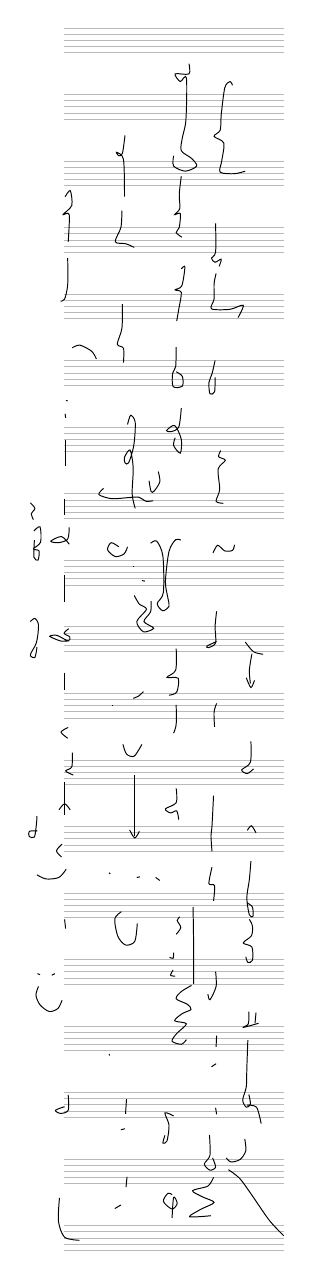
\begin{tikzpicture}[x=.0065cm,y=-.0065cm,line width=.35pt]
\foreach \a in {0,130,260,390,520,650,780,910,1040,1170,1300,1430,1560,1690,1820,1950,2080,2210,2340}{\foreach \b in {0,12,24,36,48}{\draw[gray!55,line width=.12pt] (80,{\a+\b})--(510,{\a+\b});}}
\draw plot[smooth] coordinates {(325,70) (325,90) (298,90) (308,105) (320,98) (319,180) (312,215) (310,240) (330,255) (340,270) (318,280) (295,270) (295,250)};
\draw plot[smooth] coordinates {(410,112) (405,105) (395,117) (388,170) (386,200) (374,212) (393,225) (389,260) (386,282) (414,285) (435,280)};
\draw plot[smooth] coordinates {(200,210) (195,245) (188,250) (183,243) (197,257) (199,330)};
\draw plot[smooth] coordinates {(310,290) (306,325) (307,353) (297,365) (308,363) (306,390) (300,400) (311,409)};
\draw plot[smooth] coordinates {(83,330) (93,318) (96,347) (79,365) (91,365) (89,418)};
\draw plot[smooth] coordinates {(194,357) (192,390) (181,418) (202,422) (218,429)};
\draw plot[smooth] coordinates {(377,382) (377,438) (369,450) (376,458) (388,452) (384,466)};
\draw plot[smooth] coordinates {(88,450) (88,502) (82,530) (74,534)};
\draw plot[smooth] coordinates {(310,471) (317,467) (311,504) (298,512) (310,517) (305,550) (301,573)};
\draw plot[smooth] coordinates {(378,480) (374,500) (374,530) (369,549) (405,550) (431,542) (421,566)};
\draw plot[smooth] coordinates {(195,540) (194,587) (185,618) (197,626) (197,654)};
\draw plot[smooth] coordinates {(97,625) (112,620) (135,632) (144,647)};
\draw plot[smooth] coordinates {(300,624) (299,662) (293,675) (294,701) (312,700) (312,681) (300,672)};
\draw plot[smooth] coordinates {(376,650) (370,676) (364,693) (366,715) (375,711) (376,683)};
\draw plot[smooth] coordinates {(85,728) (88,729)};
\draw plot[smooth] coordinates {(83,754) (84,762)};
\draw plot[smooth] coordinates {(205,775) (211,757) (220,771) (217,817) (207,850) (200,850) (199,839) (210,825) (216,860) (214,911) (220,939)};
\draw plot[smooth] coordinates {(310,743) (305,780) (290,789) (281,787) (297,777) (310,804) (308,831) (295,816) (298,801)};
\draw plot[smooth] coordinates {(84,806) (84,857)};
\draw plot[smooth] coordinates {(387,826) (383,838) (396,845) (382,862) (385,902) (378,925) (392,929)};
\draw plot[smooth] coordinates {(265,867) (268,887) (257,905) (251,906) (247,885)};
\draw plot[smooth] coordinates {(158,900) (149,912) (174,920) (205,918) (227,917) (241,925) (255,924)};
\draw plot[smooth] coordinates {(82,920) (82,952)};
\draw plot[smooth] coordinates {(15,928) (24,939) (17,949) (21,961)};
\draw plot[smooth] coordinates {(22,983) (34,975) (35,1005) (21,1018) (32,1022) (30,1040) (22,1034) (23,1001)};
\draw plot[smooth] coordinates {(91,976) (88,999) (70,1006) (55,1003) (76,994) (91,1009)};
\draw plot[smooth] coordinates {(188,1014) (173,1006) (166,1020) (181,1033) (198,1028) (205,1014)};
\draw plot[smooth] coordinates {(250,1007) (262,1003) (274,1032) (275,1103) (263,1125) (274,1139) (286,1130) (284,1115) (279,1082) (286,1023) (299,1000) (309,1001)};
\draw plot[smooth] coordinates {(372,1026) (381,1011) (395,1022) (410,1021) (414,1010)};
\draw plot[smooth] coordinates {(217,1051) (217,1054)};
\draw plot[smooth] coordinates {(233,1080) (239,1081)};
\draw plot[smooth] coordinates {(81,1070) (81,1121)};
\draw plot[smooth] coordinates {(218,1109) (228,1126) (242,1136) (223,1160) (236,1180) (256,1173) (237,1160) (250,1141) (251,1120)};
\draw plot[smooth] coordinates {(379,1140) (376,1170) (377,1202) (363,1211) (360,1208) (379,1199)};
\draw plot[smooth] coordinates {(15,1160) (24,1154) (31,1167) (27,1201) (15,1225) (24,1230) (28,1210)};
\draw plot[smooth] coordinates {(90,1174) (81,1183) (92,1190) (89,1198) (67,1187) (53,1189) (74,1198) (88,1198)};
\draw plot[smooth] coordinates {(435,1200) (451,1219) (470,1224)};
\draw plot[smooth] coordinates {(448,1223) (443,1255) (445,1281)};
\draw plot[smooth] coordinates {(437,1270) (446,1289) (453,1275)};
\draw plot[smooth] coordinates {(300,1213) (299,1255) (282,1269) (304,1271) (301,1298) (286,1304)};
\draw plot[smooth] coordinates {(82,1260) (82,1294)};
\draw plot[smooth] coordinates {(236,1297) (226,1306) (216,1310)};
\draw plot[smooth] coordinates {(174,1324) (177,1324)};
\draw plot[smooth] coordinates {(300,1323) (300,1361) (295,1378)};
\draw plot[smooth] coordinates {(379,1320) (374,1337) (375,1366)};
\draw plot[smooth] coordinates {(89,1367) (75,1376) (88,1388)};
\draw plot[smooth] coordinates {(196,1400) (203,1419) (218,1423) (233,1400)};
\draw plot[smooth] coordinates {(97,1416) (96,1444) (84,1452) (99,1460)};
\draw plot[smooth] coordinates {(446,1394) (445,1435) (428,1450) (439,1457) (451,1448)};
\draw plot[smooth] coordinates {(218,1460) (218,1510) (218,1580)};
\draw plot[smooth] coordinates {(209,1567) (219,1583) (228,1570)};
\draw plot[smooth] coordinates {(300,1486) (300,1514) (279,1526) (289,1534) (301,1530) (305,1547)};
\draw plot[smooth] coordinates {(82,1474) (82,1538)};
\draw plot[smooth] coordinates {(71,1528) (82,1516) (93,1528)};
\draw plot[smooth] coordinates {(28,1540) (27,1555) (23,1581) (13,1580) (13,1570) (29,1569)};
\draw plot[smooth] coordinates {(77,1595) (66,1608) (76,1620)};
\draw plot[smooth] coordinates {(85,1644) (71,1660) (46,1663) (28,1655)};
\draw plot[smooth] coordinates {(373,1500) (370,1559) (368,1579) (370,1609)};
\draw plot[smooth] coordinates {(439,1568) (447,1559) (456,1573)};
\draw plot[smooth] coordinates {(370,1640) (364,1672) (375,1676) (373,1706)};
\draw plot[smooth] coordinates {(446,1628) (443,1664) (438,1700) (443,1733) (450,1736) (449,1718) (439,1710)};
\draw plot[smooth] coordinates {(169,1651) (171,1653)};
\draw plot[smooth] coordinates {(223,1660) (229,1659)};
\draw plot[smooth] coordinates {(260,1660) (268,1666)};
\draw plot[smooth] coordinates {(193,1727) (180,1741) (186,1775) (201,1792) (219,1785) (224,1750)};
\draw plot[smooth] coordinates {(82,1742) (84,1760)};
\draw plot[smooth] coordinates {(307,1737) (302,1744) (309,1758) (300,1771)};
\draw plot[smooth] coordinates {(333,1718) (334,1789) (334,1868)};
\draw plot[smooth] coordinates {(443,1742) (449,1755) (447,1774) (431,1788) (448,1796) (449,1822) (440,1826) (436,1815)};
\draw plot[smooth] coordinates {(295,1807) (294,1818) (287,1816)};
\draw plot[smooth] coordinates {(294,1841) (289,1851) (298,1853)};
\draw plot[smooth] coordinates {(29,1848) (34,1850)};
\draw plot[smooth] coordinates {(57,1851) (63,1848)};
\draw plot[smooth] coordinates {(31,1873) (26,1890) (34,1909) (52,1922) (69,1916) (77,1900)};
\draw plot[smooth] coordinates {(330,1871) (310,1883) (300,1897) (322,1908) (329,1918) (312,1926) (297,1940) (320,1946) (301,1965) (292,1980) (310,1986) (320,1977)};
\draw plot[smooth] coordinates {(377,1844) (378,1873) (366,1899) (362,1888)};
\draw plot[smooth] coordinates {(442,1922) (441,1946) (431,1953) (461,1945)};
\draw plot[smooth] coordinates {(456,1924) (454,1945)};
\draw plot[smooth] coordinates {(379,1969) (378,1991)};
\draw plot[smooth] coordinates {(378,2024) (369,2030)};
\draw plot[smooth] coordinates {(169,2005) (170,2008)};
\draw plot[smooth] coordinates {(440,1978) (438,2034) (437,2069) (430,2095) (437,2109) (445,2103) (442,2084)};
\draw plot[smooth] coordinates {(89,2085) (89,2115) (74,2121) (64,2115) (82,2108)};
\draw plot[smooth] coordinates {(203,2093) (201,2122)};
\draw plot[smooth] coordinates {(200,2151) (192,2153)};
\draw plot[smooth] coordinates {(295,2126) (278,2120) (286,2144) (282,2175) (274,2179) (278,2164)};
\draw plot[smooth] coordinates {(377,2110) (379,2123)};
\draw plot[smooth] coordinates {(365,2163) (366,2203) (355,2220) (366,2232) (377,2226) (371,2208)};
\draw plot[smooth] coordinates {(434,2171) (436,2194) (425,2211) (407,2216) (398,2208)};
\draw plot[smooth] coordinates {(438,2105) (457,2109) (466,2141)};
\draw plot[smooth] coordinates {(204,2245) (202,2265)};
\draw plot[smooth] coordinates {(192,2300) (180,2307)};
\draw plot[smooth] coordinates {(292,2280) (284,2277) (275,2293) (292,2308) (302,2297) (295,2285) (292,2325)};
\draw plot[smooth] coordinates {(373,2246) (362,2263) (332,2272) (351,2284) (374,2295) (349,2308) (326,2323) (368,2321)};
\draw plot[smooth] coordinates {(72,2286) (70,2332) (82,2363) (111,2369)};
\draw plot[smooth] coordinates {(402,2231) (424,2248) (446,2278) (482,2330) (510,2360)};
\end{tikzpicture}}}
% crop-candidate: scan 40

Soit $A$ la sous-catégorie pleine de $C$
formée des \deleted{\unsure{\Phi}} $C^i$; elle n'est pas additive,
mais tout de même \unsure{structure|strictement} $k$-linéaire,
i.e. les $\operatorname{Hom}_A$ sont des $k$-modules, leurs
compositions est $k$-bil.

\deleted{\unsure{L}}L'existence de $(C,C^\bullet)$ satisfaisant $a)$
$b)$ est immédiate par construction ``abstraite''.
On peut aussi réaliser $C$ comme la cat. (des
complexes de chaînes \inserted{$L_*$} de $k$-modules
satisfaisant les conditions

$1^\circ)$ \deleted{\unsure{le}} $L_*$ est acyclique i.e. $H_i(L_*)=0$ $\forall i\geqslant0$.

$2^\circ)$ $L_n$ et $Z_n(L_*)$ sont libres de t.f. pour $\forall n$.

$3^\circ)$ $L_n$ est nul pour $n$ grand.

On prendra alors :
\[
C^i=\deleted{\unsure{K(C^i_*)}}C^i_*=\left\{
\begin{gathered}
\cdots\ 0\ \cdots\
\overset{\text{deg }i+1}{k}\xrightarrow{\mathrm{id}}
\overset{\text{deg }i}{k}\longrightarrow0\ \cdots\longrightarrow
\overset{\text{deg }0}{0}
\end{gathered}\right\}
\]
i.e. les comp. sont nulles sauf en degrés $i,i+1$ où
on a $k$, et l'op. diff. \unsure{$d_{i+1}$} est l'identité.
On prend $C^i_*\xrightarrow{d^i}C^{i+1}_*$ caractérisé
par $(d^i)_{i+1}=\operatorname{id}_k$. Les conditions $a)$ et $b)$ sont
satisfaites trivialement. On pourrait aussi
\unsure{prendre} des complexes de cochaînes : le plus,

\scanpage{41}
% archive foliation: 40
\deleted{
$\{C$. catégorie $\{$ des $k$-modules $\frac12$ simpliciaux \deleted{\unsure{str.}}\inserted{$L_*$} qui
sont flasques et str. $\partial$-parfaits, i.e. qui satisfont
aux deux conditions équivalentes

$a)$ $L_*$ est \deleted{isomorphe}\inserted{isomorphe} à une somme directe finie
de modules $\frac12$ simpliciaux
\[
\inserted{C^i_*=\Lambda^{i+1}\Phi_{*k}\ (i\geqslant0)}
\qquad\deleted{\unsure{\Phi(i)_*=\Lambda^i\Phi_{*k}}\ (i\geqslant1)}.
\]
\margin{\unsure{On suppose les modules proj. de type fini sur $k$ libres pour $k$ principal}.}

$b)$ les $L_n$ sont libres de type fini, de rang constant
sur $\operatorname{Spec}k$, la fonction $n\longmapsto\operatorname{rg}_kL_n$ est polynomiale
pour $n$ grand, $L_*$ est flasque i.e. $\pi_i(L_*)=0$ pour $i\geqslant0$.

$A\subset C$ la sous-catégorie pleine formée des \deleted{\unsure{\Phi(i)_*}}\inserted{$C^i_*$}.

\uline{NB}. $C$ est additive (et karoubienne), $A$ n'est pas
stable par sommes finies, mais hérite une structure
$k$-linéaire. On a
\[
\operatorname{Hom}(\deleted{\unsure{\Phi}}C^i_*,\deleted{\unsure{\Phi}}C^j_*)=
\begin{cases}
0&\text{si }j\ne i,i+1\\
k&\text{si }j=i,\ \text{base }\operatorname{id}_{(C^i)}\\
k&\text{si }j=i+1,\ \text{base }d^i=T_*\wedge
\end{cases}
\]
Notons que
\deleted{\unsure{\Phi(i)_*=C^{i-1}_*\ (i\geqslant1),\qquad C^i_*=\Phi(i+1)_*\ (i\geqslant0)}}

$C^\bullet_*=(C^i_*,T_*\wedge)$ est un complexe de cochaînes dans
$A$ ou dans $C$ ou dans $\widehat\Delta_{k\text{-}lin}$ --- il jouera
le rôle du complexe de cochaînes \uline{universel}.
}

\deleted{\unsure{En effet}}
\uline{Prop. 1} Soit $B$ une catégor. \deleted{additive}\inserted{$k$-additive}. Alors
\diagram{\begin{tikzcd}[column sep=large,row sep=large]
\underline{\operatorname{Hom}}_{\unsure{add\,k|additif}}(C,B)
\arrow[r,"{\mathrm{res}}","\simeq"']&
\underline{\operatorname{Hom}}_{k\text{-}lin}(A,B)\arrow[d,"{F\longmapsto F(C^\bullet_*)}","\simeq"']\\
& B^\bullet_k=\text{cat. des \inserted{complexes de} cochaînes de }B
\end{tikzcd}}
\deleted{\uline{\unsure{Assertion}} Soit $E^\bullet\in\operatorname{Ob}B^\bullet$ un complexe de cochaînes
de $B$.}

\uline{Exemple 1} \inserted{Faisons $B=\mathrm{Ab}_k$.} Soit $L_*\in\operatorname{Ob}C$, considérons le
foncteur cov. qu'il représente
\[
C\longrightarrow\mathrm{Ab}_k:\quad M_*\longmapsto\operatorname{Hom}_C(L_*,M_*).
\]
On a ainsi un foncteur pl. fid (\unsure{nature des fonct. repr.} $\ldots$)
\diagram{\begin{tikzcd}[column sep=small,row sep=small]
C^\circ\arrow[r,hook]&\underline{\operatorname{Hom}}_{k\text{-}lin}(C,\mathrm{Ab}_k)\arrow[dr,"\simeq"]&&\\
&&\underline{\operatorname{Hom}}_{\unsure{k\text{-}lin|add}}(A,\mathrm{Ab}_k)\arrow[r,"\simeq"]&\mathrm{Ab}^{\bullet}_{k}
\end{tikzcd}}

\scanpage{42}
% archive foliation: 41
On trouve donc un foncteur pl. fid
\[
C^\circ\lhook\joinrel\xrightarrow{\deleted{\unsure{\beta}}\alpha^\bullet}\mathrm{Ab}^\bullet_k\deleted{\unsure{*}},
\]
qui associe à tout \deleted{\unsure{M_*}} $L_*$ associe le complexe
de cochaînes $\operatorname{Hom}_C(L_*,C^\bullet_*)$
\diagram{\begin{tikzcd}[column sep=small]
0\arrow[r]&\operatorname{Hom}(L_*,C^0_*)\arrow[r]&\operatorname{Hom}(L_*,C^1_*)\arrow[r]&\cdots
\end{tikzcd}}
et dont la restriction à $A$ est donnée par
\[
\alpha^\bullet\deleted{\unsure{\beta}}(C^i_*)=\left(0\longrightarrow0\longrightarrow\cdots\ 0\longrightarrow
\underset{\text{degré }i}{k}\xrightarrow{\mathrm{id}}
\underset{\text{degré }i+1}{k}\longrightarrow0\longrightarrow\cdots\right)
=\deleted{\unsure{K}}\inserted{C'_i},
\]
et par la loi
\diagram{\begin{tikzcd}[row sep=small,column sep=large]
&\alpha^\bullet(C^i_*)\arrow[d,equal]&\alpha(C^{i+1}_*)\arrow[l,"\alpha^\bullet(d^i)"']\arrow[d,equal]\\
&\unsure{(C'_i)^\bullet|K'_i}\arrow[r]&\unsure{(C'_{i+1})^\bullet|K'_{i+1}}\\
&\vdots&\vdots\\
&0\arrow[d]&0\arrow[d]\\
&k\arrow[d]&0\arrow[l]\arrow[d]\\
i+1&k\arrow[d]&k\arrow[l,leftrightarrow,"\mathrm{id}"']\arrow[d]\\
i+2&0\arrow[d]&k\arrow[l]\arrow[d]\\
&0&0\\
&\vdots&\vdots
\end{tikzcd}}
\[
k\longrightarrow0
\]
\margin{L'image essentielle \inserted{d'$\alpha^\bullet$} de $C^\circ$
est la catégor. des $K^\bullet\in\operatorname{Ob}\mathrm{Ab}_k^\bullet$
qui sont libres de t.f.
en ttes dimensions, et
qui sont à \unsure{ch.} nulle
(on admettra que tt facteur
direct d'un libre de t.f.
est libre).}

\margin{\unsure{Commencer} par Ex 2}
\uline{Ex 2} Faisons $B=\mathrm{Ab}_k^\circ$,
qui est $k$-linéaire (on suppose
$k$ commutatif), et pour $\forall L_*\in\operatorname{Ob}C$, on consi-
dère le foncteur controv. qu'il représente, \unsure{interprété}
comme foncteur $k$-lin.
\[
C^\circ\longrightarrow\deleted{\unsure{\mathrm{Ab}^\circ_k}}\mathrm{Ab}_k^{\unsure{\circ|\bullet}}:
\quad M_*\longmapsto\operatorname{Hom}_C(M_*,L_*)
\]
on trouve ainsi un foncteur pl. fid (pour la
même raison)
\diagram{\begin{tikzcd}[column sep=small,row sep=large]
C\arrow[r,hook]&\underline{\operatorname{Hom}}_{k\text{-}lin}(C^\circ,\mathrm{Ab}_k^{\unsure{\circ|\bullet}})\arrow[r,"\simeq"]\arrow[d,"\simeq"']&
\underline{\operatorname{Hom}}_{k\text{-}lin}(C,\mathrm{Ab}_k^\circ)^\circ\arrow[d,"\simeq"]\\
&\underline{\operatorname{Hom}}_{k\text{-}lin}(A^\circ,\mathrm{Ab}_k^{\unsure{\circ|\bullet}})\arrow[r,"\simeq"]\arrow[d]&
\underline{\operatorname{Hom}}_{k\text{-}lin}(A,\mathrm{Ab}_k^\circ)^\circ\arrow[d,"\simeq"]\\
&\unsure{\{(\mathrm{Ab}_k^\circ)_*\simeq\deleted{\mathrm{Ab}_{k*}}^{*}\}^{\circ}}&
(\mathrm{Ab}_k^{\circ\unsure{*|\bullet}})^\circ
\end{tikzcd}}
on trouve un foncteur pl. fid.
\[
C^{\unsure{\circ}}\lhook\joinrel\xrightarrow{\beta}\mathrm{Ab}_{k*}.
\]

\scanpage{43}
% archive foliation: 42
On trouve que
\[
\beta_*(C^i)=\deleted{\unsure{C_{i*}}}
(\cdots0\longrightarrow\cdots\ 0\longrightarrow
\overset{\unsure{i}}{k}\longrightarrow\overset{\unsure{i-1}}{k}\longrightarrow0\longrightarrow\cdots\longrightarrow0)
\quad\inserted{\text{pour }i\geqslant1},
\]
\[
\inserted{\beta_*(C^0)=(\cdots\underset{\unsure{\text{degr }0}}{\deleted{\unsure{k}}}\longrightarrow0\longrightarrow\underset{\text{deg }0}{k}\longrightarrow0)}
\]
et $\beta_*(d^i):C^i_*\xrightarrow{d^i}C^{i+1}_*$
est donné par
\[
(d^i)_{\unsure{i|i+1}}=\operatorname{id}_k\qquad i\geqslant0.
\]
\deleted{\unsure{On désignera désormais par} \inserted{$K_*$} la cat. des
complexes de chaînes \unsure{et ceci nous donne}
\unsure{une autre possibilité de construction}
d'un couple $(C,C^\bullet)$.}
\margin{\unsure{Ce n'est pas}\ \unsure{très bon}\ \unsure{de commencer}\
\unsure{à l'intégralité}\ \illegible{2}\ \unsure{pour}\ \unsure{fonctorialité}.}

\uline{Passage de l'exemple 1 à l'exemple 2}

Considérons le foncteur
\[
M\longmapsto M^\vee\qquad
\mathrm{Ab}_k^\circ\longrightarrow\mathrm{Ab}_k
\]
\margin{\figure{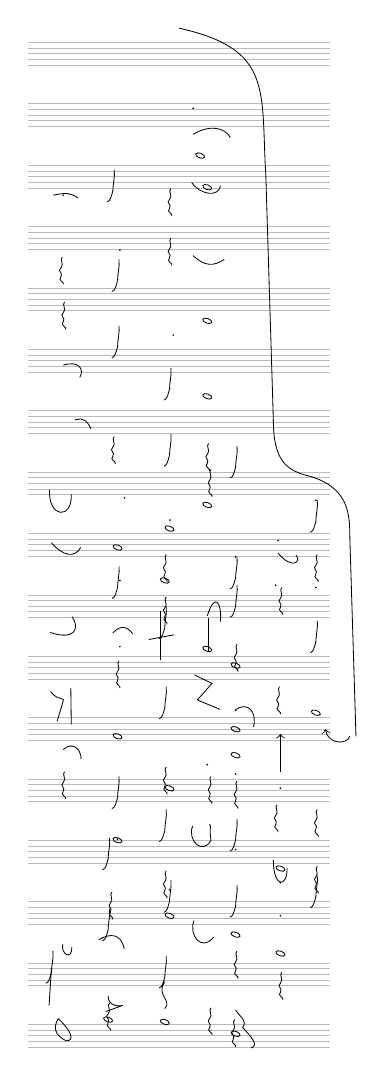
\begin{tikzpicture}[x=.006cm,y=-.006cm,line width=.3pt]
\foreach \a in {0,130,260,390,520,650,780,910,1040,1170,1300,1430,1560,1690,1820,1950,2080}{\foreach \b in {0,12,24,36,48}{\draw[gray!55,line width=.12pt](0,{\a+\b})--(640,{\a+\b});}}
% Separate manually positioned pen strokes, respecting the visible columns and row offsets.
\foreach \x/\y in {180/315,190/505,190/645,300/735,300/875,440/900,610/1015,190/1155,290/1240,440/1135,440/1195,610/1270,290/1410,190/1600,290/1670,440/1690,170/1730,300/1820,440/1830,610/1810,170/1880,50/1970,290/1980}{\draw(\x,\y) .. controls(\x,{\y-15}) and({\x+5},{\y-30})..({\x+3},{\y-45});\draw(\x,\y).. controls({\x-3},{\y+10}) and({\x-5},{\y+22})..({\x-12},{\y+23});}
\foreach \x/\y in {300/325,300/430,70/470,75/565,180/850,380/865,385/920,290/1100,610/1100,290/1190,535/1170,440/1290,190/1325,530/1380,290/1550,75/1560,385/1570,440/1580,525/1630,610/1640,290/1770,610/1760,175/1815,440/1940,535/1985,385/2060,435/2085,170/2050}{\draw({\x+3},{\y-15})..controls({\x-4},{\y-10})and({\x+8},\y)..(\x,{\y+8})..controls({\x-9},{\y+15})and({\x+6},{\y+18})..(\x,{\y+27})..controls({\x-8},{\y+34})and({\x+9},{\y+39})..({\x+5},{\y+43});}
\foreach \x/\y in {365/240,380/307,380/590,380/750,380/980,300/1030,190/1070,290/1140,380/1285,440/1320,610/1420,440/1455,190/1470,440/1510,300/1580,190/1690,535/1750,300/1850,440/1890,535/1930,170/2070,290/2075,440/2100}{\draw[rotate around={-20:(\x,\y)}](\x,\y)ellipse(10 and 5);}
\foreach \x/\y in {350/140,75/324,195/440,308/620,205/965,610/970,301/1012,530/1055,440/1090,195/1140,525/1150,610/1155,195/1280,440/1415,535/1470,380/1530,440/1550,535/1580,190/1688,440/1710,300/1795,535/1780,535/1850}{\fill(\x,\y)circle(2);}
\draw(350,195)..controls(385,174)and(417,180)..(429,202);
\draw(54,324)..controls(80,318)and(92,319)..(106,330);
\draw(347,297)..controls(363,322)and(404,330)..(408,304);
\draw(350,452)..controls(375,475)and(393,475)..(416,460);
\draw(75,684)..controls(106,674)and(121,691)..(110,710);
\draw(100,800)..controls(120,793)and(127,805)..(134,819);
\draw(46,948)..controls(43,1009)and(95,1011)..(92,957);
\draw(50,1060)..controls(76,1090)and(100,1092)..(112,1070);
\draw(530,1082)..controls(560,1118)and(580,1100)..(568,1086);
\draw(47,1250)..controls(101,1268)and(110,1240)..(94,1217);
\draw(180,1251)..controls(199,1231)and(213,1240)..(222,1253);
\draw(280,1205)--(280,1308);\draw(256,1265)--(310,1255);
\draw(380,1215)..controls(395,1166)and(411,1183)..(408,1227);\draw(382,1220)--(382,1290);
\draw(48,1375)..controls(67,1400)and(80,1380)..(73,1402)--(62,1438);\draw(91,1368)--(92,1445);
\draw(353,1340)--(390,1358)--(359,1393)--(407,1413);
\draw(440,1414)..controls(465,1395)and(486,1418)..(478,1450);
\draw(75,1498)..controls(94,1481)and(112,1495)..(113,1518);
\draw[->](535,1545)--(535,1465);
\draw(349,1660)..controls(337,1690)and(370,1723)..(388,1690)..controls(384,1670)and(389,1658)..(385,1656);
\draw(520,1732)..controls(520,1792)and(550,1792)..(549,1748);
\draw(74,1910)..controls(69,1931)and(94,1946)..(93,1916);
\draw(352,1860)..controls(340,1890)and(367,1928)..(394,1895);
\draw(150,1901)..controls(172,1888)and(197,1885)..(204,1920);
\draw(64,2068)..controls(89,2090)and(102,2115)..(81,2115)..controls(56,2102)and(54,2087)..(64,2068);
\draw(50,1960)--(45,2040);\draw(290,1990)..controls(270,2018)and(307,2029)..(290,2047);
\draw(170,2020)..controls(170,2043)and(196,2042)..(201,2040)--(165,2053);
\draw(440,2050)..controls(452,2067)and(465,2072)..(455,2087)..controls(480,2113)and(487,2125)..(473,2130);
\draw(320,-30)..controls(520,15)and(493,100)..(504,280)--(520,800)..controls(520,890)and(550,908)..(600,920)..controls(680,945)and(682,1000)..(682,1050)--(695,1470);
\draw[->](682,1470)..controls(674,1490)and(635,1485)..(630,1455);
\end{tikzpicture}}}
% crop-candidate: scan 43

qui induit une équivalence de la catégorie
des \inserted{$k$-}modules libres de t.f. avec elle-même.
Cela donne aussi une équivalence entre
les cat. des complexes de chaînes et cochaînes
à comp. \deleted{\unsure{K_*=K^\vee}} libres de t.f., et entre
celles où les $Z_n$ (et $Z^i$) sont libres de t.f. et \unsure{bornées}.
\deleted{\unsure{On peut donc}\ \unsure{supposer}\ \unsure{les deux équivalences}\
\unsure{et on peut les composer}.}
\deleted{\unsure{On a donc}\ \unsure{par}\ $\alpha^\bullet_*(K)$\ \unsure{et}\ $(\alpha^{\unsure{\bullet|'}})^\vee$}
un diagramme d'équivalences
\diagram{\begin{tikzcd}[row sep=large,column sep=large]
\deleted{\unsure{K_*}}\ C\arrow[r,"\alpha_*","\simeq"']\arrow[d,"(\alpha^{\unsure{\bullet|'}})^\circ"',"\simeq"]&K_*\arrow[dl,"\simeq"]\\
K^{\bullet\circ}&
\end{tikzcd}}
\deleted{\unsure{Les deux définissent une même}\ \unsure{dualité}\
\unsure{en particulier}\ \unsure{à $A$}\ \unsure{ce qui est trivial}.}

\uline{\unsure{Explicitons quand même}}

\uline{Prop. 2} On a une dualité parfaite fonctorielle
en $M\in\operatorname{Ob}K_*$ (et \unsure{vice versa})
\diagram{\begin{tikzcd}[column sep=small,row sep=small]
\alpha_{\unsure{k|*}}(M)_{\unsure{n|i}}\arrow[d,equal]&\mathbin{\times}&
\alpha^{\unsure{n|i}}(M)\arrow[d,equal]\arrow[r]&k\arrow[d,"\simeq"]\\
\operatorname{Hom}(C^{\unsure{n|i}}_*,\unsure{M|k})&\mathbin{\times}&
\operatorname{Hom}(M,C^{\unsure{n|i}}_*)\arrow[r,"{\text{par }\circ}"']&
\operatorname{Hom}(C^{\unsure{n|i}}_*,C^{\unsure{n|i}}_*)\arrow[r,"\simeq"]&k
\end{tikzcd}}

\scanpage{44}
% archive foliation: 43
Revenons à la prop. 1. Soit $C^\bullet$ \inserted{$\in\operatorname{Ob}B^\bullet$} un complexe
de cochaînes de $B$, comment reconstituer
le foncteur $k$-lin
\[
F_C:\unsure{K|C}\longrightarrow B
\]
i.e. comment ``calculer'' $F_C(x)$ pour $x\in\operatorname{Ob}\unsure{K|C}$ ?
Il faut bien sûr commencer par ``repérer'' $x$,
disons par $\alpha^\bullet(x)\in\mathrm{Ab}_k^\bullet$. Ceci dit, on trouve

\uline{Prop. 3}. On a un isom. bifonctoriel en $F,x$
(si $F\in\deleted{\unsure{F}}\operatorname{Ob}\underline{\operatorname{Hom}}_{k\text{-}lin}(C,B)$)
\[
\begin{gathered}
F(x)\xrightarrow{\sim}\operatorname{Hom}^\bullet_k(\alpha^\bullet(x),F(C^\bullet))\\
\operatorname{Hom}^\bullet_k(\overset{\text{''}}{\alpha^\bullet(x)},C^\bullet_F),
\end{gathered}
\]
[où on définit, pour un $K^\bullet\in\operatorname{Ob}\mathrm{Ab}_k^\bullet$ et
$C^\bullet\in\operatorname{Ob}B_k^\bullet$, l'objet $\operatorname{Hom}^\bullet_k(K^\bullet,C^\bullet)$ de $B$
(s'il existe) par l'isom. fonctoriel en $b\in\operatorname{Ob}B$
\[
\operatorname{Hom}_{\inserted{B}}(b,\operatorname{Hom}^\bullet(K^\bullet,C^\bullet))
\simeq\operatorname{Hom}_{B^\bullet}(b\otimes_k K^\bullet,C^\bullet).
\]
Si les $K^i$ sont libres de type fini, $b\otimes_k K^\bullet$
est bien défini, donc $b\longmapsto\operatorname{Hom}_{B^\bullet}(b\otimes_k K^\bullet,C^\bullet)$
l'est, et la question est si ce foncteur est
représentable; il se trouve qu'il l'est si
$K^\bullet$ \deleted{\unsure{est}} \deleted{\unsure{plein}} $\unsure{=|\subset}\in\operatorname{Ob}\deleted{\unsure{\mathrm{Ab}_k^\bullet}}K^\bullet$ [ Mais de façon
générale, c'est le sous-foncteur de
\[
\prod_i\underset{\in\operatorname{Ob}B}{\operatorname{Hom}_k(K^i,C^i)}
\]
noyau de
\[
\prod_i\operatorname{Hom}_k(K^i,C^i)\mathrel{\substack{\xrightarrow{\delta}\\[-.4ex]\deleted{\unsure{\longleftarrow|\longrightarrow}}}}
\prod_i\operatorname{Hom}_k(K^i,C^{i+1})
\]
($\delta(u^i)=du^i-u^{i+1}d$) --- \uline{ceci est repr.} si
$B$ \deleted{\uline{abélienne}}\inserted{stable par Ker}, si les $\operatorname{Hom}_k(K^i,C^i)$ sont
repr. (p.ex. les $K^i$ de prés. finie) et les deux
\margin{\unsure{remettre avant énoncé prop. 3}}
